%% main_tcc_uemg.tex v1.0, Milton Miranda Neto
% adaptado de modeloABNT2.tex, v1.0
% ------------------------------------------------------------------------
% ------------------------------------------------------------------------
% eesc: Modelo de Trabalho Acadêmico (tese de doutorado, dissertação de
% mestrado e trabalhos monográficos em geral) em conformidade com
% ABNT NBR 14724:2011.
% ------------------------------------------------------------------------
% ------------------------------------------------------------------------
% Atualizações.
% 24/01/2019 - Adaptação para a UEMG.

% ------------------------------------------------------------------------
% Opções:
% 	tesedr:     Formata documento para tese de doutorado
%	qualidr:    Formata documento para qualificação de doutorado
% 	dissertmst: Formata documento para dissertação de mestrado
% 	qualimst:   Formata documento para qualificação de mestrado
%   tccgrad:    Formata documento para tcc de graduação
% ------------------------------------------------------------------------
\documentclass[tccgrad]{tccUEMG}
%Não altere o comando seguinte. O título de seu trabalho será especificado mais adiante.
\title{Template TCC UEMG}

% ---
% PACOTES
% ---

% ---
% Pacotes fundamentais
% ---
\usepackage{cmap}				% Mapear caracteres especiais no PDF
\usepackage{lmodern}				% Usa a fonte Latin Modern
\usepackage{makeidx}            	% Cria o indice
\usepackage{hyperref}  			% Controla a formação do índice
\usepackage{lastpage}			% Usado pela Ficha catalográfica
\usepackage{indentfirst}			% Indenta o primeiro parágrafo de cada seção.
\usepackage{nomencl} 			% Lista de simbolos
\usepackage{graphicx}			% Inclusão de gráficos
\usepackage{pdflscape}			% Páginas horizontais para figuras largas
% ---

% ---
% Pacotes adicionais, usados apenas no âmbito do Modelo eesc
% ---
\usepackage{lipsum}				       % para geração de dummy text
\usepackage[printonlyused]{acronym}
\usepackage[table]{xcolor}
% ---


% ---
% Informações de dados para CAPA e FOLHA DE ROSTO
% ---
%
% Título:
%	1. Título em português
%	2. Título em inglês
\titulo{APLICAÇÃO DE ENGENHARIA DE DADOS E BUSINESS INTELLIGENCE NA ANÁLISE DE INDICADORES EDUCACIONAIS DA EDUCAÇÃO BÁSICA BRASILEIRA}{Application of Data Engineering and Business Intelligence in the Analysis of Educational Indicators of Brazilian Basic Education}
%
% Autor:
%	1. Nome completo do autor
%	2. Formato de nome para bibliografia
\autor{Milton Rafael De Souza Garcia}{Souza Garcia, Milton}
%
% Cidade
\local{Ituiutaba}
% Ano de defesa
\data{2026}
% Área de concentração da pesquisa
\areaconcentracao{Sistemas de Informação}
% Nome do orientador
\orientador{Anderson de Melo Valadão}
% Nome do coorientador
%\coorientador{Nome completo do coorientador}
% ---

% ---
% compila o indice
% ---
\makeindex
% ---

% ---
% Compila a lista de abreviaturas e siglas
% ---
\makenomenclature
% ---

% ---
% Inserir ficha catalográfica
%
% Caso o comando \inserirfichacatalografica seja definido, a %ficha catalográfica
% será inserida atrás da folha de rosto. Caso contrário a página será deixada em
% branco.
%
% CUIDADO: Esta opção deve ser preenchida antes do comando \maketitle
% ---
%entre em contato com a biblioteca para obter a sua ficha catalográfica em arquivo pdf. Essa %folha só será inserida no documento após a sua defesa.

%\inserirfichacatalografica{elementos/fichaCatalografica.pdf}
% ---

% ---
% Inserir folha de aprovação
%
% Caso o comando \inserirfolhaaprovacao seja definido, a a folha de aprovação
% será inserida. Além disso, conforme Resolução CoPGr 5890, as informações
% de rodapé são inseridas apropriadamente na folha de rosto.
%
% CUIDADO: Esta opção deve ser preenchida antes do comando \maketitle
% ---
% baseie-se no modelo desse documento e gere a sua folha de %rosto em arquivo pdf.

%\inserirfolhaaprovacao{}
% ---

% ----
% Início do documento
% ----

\begin{document}

% ----------------------------------------------------------
% ELEMENTOS PRÉ-TEXTUAIS
% ----------------------------------------------------------
\pretextual

% ---
% Insere Capa, Folha de rosto, Ficha catalográfica (se inserida)
% e folha de aprovação (se inserida).
% ---
\maketitle


% ---
% Dedicatória
% ---
\imprimirdedicatoria{Dedico este trabalho à minha esposa, Alane de Cássia Alves Ferreira, professora e inspiração desta pesquisa.
Seu apoio, sua confiança e sua presença foram essenciais em minha caminhada acadêmica. Minha formação é, em grande parte, fruto do seu incentivo, do seu cuidado e da força que você sempre me transmitiu.
Esta conquista também pertence a você.
}
% ---

% ---
% Agradecimentos
% ---
\imprimiragradecimentos{
Agradeço, primeiramente, a Deus, pela força, saúde e perseverança concedidas ao longo desta caminhada.

À minha esposa, Alane de Cássia Alves Ferreira, professora, companheira e inspiração deste trabalho, agradeço pelo apoio constante, pelo incentivo nos momentos difíceis e por acreditar em mim. Sua presença foi essencial para que eu chegasse até aqui.
Agradeço à minha família, pelo apoio, pela compreensão e por fazer parte da minha trajetória de vida e formação.

Ao meu professor orientador, Anderson, agradeço pela orientação, pelas contribuições e pelo acompanhamento durante o desenvolvimento deste trabalho.

Aos professores da Universidade do Estado de Minas Gerais — UEMG, especialmente aos docentes do curso de Sistemas de Informação, agradeço pelos conhecimentos compartilhados ao longo da minha formação acadêmica. Cada disciplina, orientação, diálogo e desafio proposto contribuiu para a construção dos saberes que tornaram possível a realização deste trabalho.

Por fim, agradeço à Universidade do Estado de Minas Gerais — UEMG, pela oportunidade de formação e por fazer parte desta importante etapa da minha vida acadêmica e profissional.
}
% ---

% ---
% Epígrafe
% ---
\imprimirepigrafe{
		“Sem dados, você é apenas mais uma pessoa com uma opinião.”\\
        W. Edwards Deming
}
% ---

% ---
% RESUMO e ABSTRACT
% ---

% Resumo em português - as palavras entre chaves são as palavras-chave do trbalho
\begin{resumo}{Engenharia de Dados. Pipelines de Dados. Indicadores Educacionais. Reprodutibilidade de Dados. Business Intelligence}

Este trabalho tem como objetivo desenvolver e analisar uma arquitetura reprodutível de Engenharia de Dados e Business Intelligence para integrar indicadores educacionais da Educação Básica brasileira. Foram utilizadas bases públicas do Instituto Nacional de Estudos e Pesquisas Educacionais Anísio Teixeira (INEP): Índice de Desenvolvimento da Educação Básica (IDEB), Sistema de Avaliação da Educação Básica (SAEB), Taxas de Rendimento Escolar, Taxa de Distorção Idade-Série (TDI) e, como análise complementar, Prova Nacional Docente (PND) 2025. A metodologia implementou em Python um pipeline de extração, transformação e carga organizado nas camadas Raw, Bronze, Silver e Gold, com auditorias, validações de qualidade, inventário das fontes e hashes SHA-256 para identificação dos insumos. A Gold foi estruturada como modelo dimensional e disponibilizada em arquivos Parquet consumidos pelo Power BI, no qual foram definidos os relacionamentos, as medidas DAX e os dashboards. A análise histórica foi padronizada em nível de Unidade Federativa para o período de 2007 a 2023, considerando IDEB, SAEB, Rendimento Escolar e TDI; a PND foi analisada separadamente em 2025. O processo resultou em cinco tabelas fato, cinco dimensões e controles de qualidade sobre esquema, domínio, cobertura temporal, duplicidade, integridade referencial e correspondência entre as camadas. Os resultados mostram que a arquitetura permite integrar fontes heterogêneas, preservar a rastreabilidade das transformações e disponibilizar dados consistentes para exploração analítica. Conclui-se que a combinação entre pipeline reprodutível e Business Intelligence contribui para transformar bases públicas dispersas em informações estruturadas e verificáveis, sem atribuir causalidade às relações observadas.

\end{resumo}

% Resumo em inglês
\begin{abstract}{Data Engineering. Data Pipelines. Educational Indicators. Data Reproducibility. Business Intelligence}

This work aims to develop and analyze a reproducible Data Engineering and Business Intelligence architecture for integrating educational indicators of Brazilian Basic Education. Public datasets from the National Institute for Educational Studies and Research Anísio Teixeira (INEP) were used: the Basic Education Development Index (IDEB), the Basic Education Assessment System (SAEB), School Flow Rates, the Age-Grade Distortion Rate (TDI), and, as a complementary analysis, the 2025 National Teacher Exam (PND). The methodology implemented a Python extract, transform, and load pipeline organized into Raw, Bronze, Silver, and Gold layers, with audits, data quality validations, a source inventory, and SHA-256 checksums for input identification. The Gold layer was structured as a dimensional model and stored in Parquet files consumed by Power BI, where relationships, DAX measures, and dashboards were defined. The historical analysis was standardized at the Federative Unit level for the 2007--2023 period, covering IDEB, SAEB, School Flow Rates, and TDI; PND was analyzed separately for 2025. The process produced five fact tables, five dimensions, and quality controls for schema, domain, temporal coverage, duplicates, referential integrity, and agreement between layers. The results show that the architecture integrates heterogeneous sources, preserves transformation traceability, and provides consistent data for analytical exploration. It is concluded that combining a reproducible pipeline with Business Intelligence helps transform scattered public datasets into structured and verifiable information, without assigning causality to the observed relationships.

\end{abstract}
% ---

% ---
% inserir lista de ilustrações
% ---
\listailustracoes
% ---

% ---
% inserir lista de tabelas
% ---
\listatabelas
% ---

% ---
% inserir lista de abreviaturas e siglas
% ---
%\listasiglas{elementos/abrev/Abreviaturas}
% ---

% ---
% inserir o sumario
% ---
\sumario
% ---

% ----------------------------------------------------------
% ELEMENTOS TEXTUAIS
% ----------------------------------------------------------
\mainmatter

% ----------------------------------------------------------
% Introdução
% ----------------------------------------------------------
\chapter[Introdução]{Introdução}

Nas últimas décadas, a produção e o armazenamento de dados passaram a ocupar papel central em diferentes áreas da sociedade. Entretanto, a disponibilidade de grandes volumes de dados, por si só, não garante sua transformação em informação útil ou conhecimento. \citeonline{loh2014bi} distingue dados, informação e conhecimento e destaca que sistemas de informação e processos de Business Intelligence podem apoiar a tomada de decisão ao organizar, analisar e contextualizar os dados disponíveis. Nesse contexto, torna-se necessário aplicar técnicas capazes de coletar, preparar, integrar, tratar e apresentar informações de maneira compreensível e analiticamente útil.

No contexto educacional brasileiro, essa realidade também se faz presente. O Instituto Nacional de Estudos e Pesquisas Educacionais Anísio Teixeira (INEP) disponibiliza diferentes bases públicas relacionadas à Educação Básica, entre elas o Índice de Desenvolvimento da Educação Básica (IDEB) \cite{inep2024ideb}, o Sistema de Avaliação da Educação Básica (SAEB) \cite{inep2025saeb}, as Taxas de Rendimento Escolar \cite{inep2025rendimento} e a Taxa de Distorção Idade-Série (TDI) \cite{inep2026tdi}. Em conjunto, essas fontes permitem observar dimensões como desempenho dos estudantes, fluxo escolar, aprovação, reprovação, abandono e distorção idade-série. Além desses indicadores históricos, este trabalho também considera a Prova Nacional Docente (PND) 2025 como base complementar de análise \cite{inep2025pnd}, especialmente por permitir observar informações relacionadas ao desempenho de participantes em diferentes áreas de formação docente.

Apesar da relevância dessas informações, sua utilização ainda apresenta desafios. Os dados encontram-se distribuídos em diferentes arquivos, períodos históricos, formatos e estruturas. Além disso, as bases possuem nomenclaturas, códigos e formas de organização distintas, o que dificulta análises integradas entre indicadores, anos, unidades federativas, redes de ensino, etapas escolares e demais categorias de análise. As fontes também variam quanto ao nível de agregação e à forma de apresentação. Neste trabalho, foram priorizados resultados oficiais agregados por Unidade Federativa sempre que disponíveis; microdados e arquivos em outros níveis foram preservados para auditoria ou empregados quando necessários. Assim, uma análise mais ampla da Educação Básica exige não apenas acesso aos dados, mas também processos consistentes de preparação, transformação, validação e modelagem.

Diante desse cenário, este trabalho delimita-se à análise da aplicação de técnicas de Engenharia de Dados e Business Intelligence na integração e visualização de indicadores educacionais brasileiros disponibilizados pelo INEP, considerando o período de 2007 a 2023 para as bases históricas de IDEB, SAEB, Rendimento Escolar e Distorção Idade-Série. A PND 2025 foi incorporada como base complementar, não compondo a série histórica principal, mas ampliando as possibilidades de análise por meio de informações relacionadas às notas, acertos, áreas de formação e códigos dos municípios de aplicação da prova.

A pesquisa concentra-se na organização das bases de IDEB, SAEB, Rendimento Escolar, Distorção Idade-Série e PND 2025, com a finalidade de compreender como essas informações podem ser estruturadas em um ambiente analítico capaz de favorecer interpretações históricas, comparativas e visuais. Para garantir maior consistência entre as bases, a análise histórica foi padronizada principalmente em nível de Unidade Federativa (UF), contemplando Anos Iniciais e Anos Finais do Ensino Fundamental. O Ensino Médio não compôs o recorte analítico desenvolvido neste trabalho.

A relevância deste estudo está no fato de que dados educacionais públicos, quando analisados de forma isolada ou fragmentada, podem limitar a compreensão da realidade educacional. Ao integrar diferentes indicadores em uma mesma estrutura analítica, torna-se possível observar relações entre desempenho, fluxo escolar, atraso escolar e desempenho em avaliações externas, contribuindo para uma leitura mais ampla da Educação Básica brasileira. Dessa forma, o trabalho busca demonstrar como técnicas computacionais podem auxiliar na transformação de dados públicos dispersos em informações organizadas, acessíveis e úteis para análise.

\section{Motivação}

A motivação para o desenvolvimento deste trabalho surgiu da percepção de que, embora o Brasil disponha de uma quantidade significativa de dados educacionais públicos, esses dados nem sempre são facilmente compreendidos ou explorados de maneira integrada. Muitas vezes, os arquivos disponibilizados exigem tratamento prévio, conhecimento técnico e organização adequada para que possam ser utilizados em análises comparativas. Essa necessidade de preparação é coerente com \citeonline{loh2014bi}, que ressalta que a quantidade de dados não é suficiente para uma análise de qualidade: os dados precisam apresentar qualidade e estar organizados em formato adequado ao processo analítico.

No campo educacional, IDEB, SAEB, Rendimento Escolar e Distorção Idade-Série permitem acompanhar dimensões distintas da Educação Básica, como desempenho em avaliações externas, fluxo escolar e distorção idade-série \cite{inep2024ideb,inep2025saeb,inep2025rendimento,inep2026tdi}. Quando analisados separadamente, esses indicadores oferecem recortes específicos da realidade educacional; sua integração, no escopo deste trabalho, permite colocá-los em uma mesma estrutura analítica e observar conjuntamente desempenho, aprovação, reprovação, abandono e atraso escolar. A inclusão da PND 2025 como base complementar também possibilita observar informações relacionadas ao desempenho de participantes em áreas de formação docente \cite{inep2025pnd}, acrescentando uma dimensão recente ao conjunto de análises realizadas.

Estudos anteriores já apontam a importância do uso de técnicas computacionais no tratamento de dados educacionais. \citeonline{soares2021} evidenciam o potencial das bases do INEP para pesquisas relacionadas à mineração e análise de dados educacionais. \citeonline{ilha2021} demonstram a relevância da construção de um Data Warehouse para organização de indicadores educacionais, enquanto \citeonline{wanderley2021} destaca o uso de Business Intelligence na visualização de informações da Educação Básica por meio de dashboards.

Apesar dessas contribuições, ainda existem desafios relacionados à integração de múltiplas bases públicas, à padronização de dados históricos e à construção de modelos analíticos que permitam analisar diferentes dimensões da Educação Básica em conjunto. Nesse sentido, este trabalho parte da necessidade de investigar como a Engenharia de Dados e o Business Intelligence podem contribuir para organizar, integrar e interpretar indicadores educacionais brasileiros de maneira mais acessível e estruturada.

\section{Objetivos e Desafios da Pesquisa}

O principal desafio desta pesquisa está na complexidade de trabalhar com diferentes bases públicas educacionais, que apresentam formatos, estruturas, períodos e categorias variadas. A integração dessas informações exige processos de extração, limpeza, transformação, padronização, validação e modelagem, de modo que os dados possam ser analisados de forma conjunta e coerente. A questão que orienta o trabalho é: como uma arquitetura reprodutível de Engenharia de Dados pode integrar bases educacionais heterogêneas do INEP e disponibilizá-las de forma consistente para análise no Power BI?

Dessa forma, o objetivo geral deste trabalho é desenvolver e avaliar um pipeline reprodutível de Engenharia de Dados, integrado a uma solução de Business Intelligence, para organizar, validar e disponibilizar indicadores educacionais brasileiros do INEP no período de 2007 a 2023, com análise complementar da PND 2025.

Para alcançar esse objetivo geral, foram definidos os seguintes objetivos específicos:\\

a) investigar as características das bases públicas educacionais disponibilizadas pelo INEP, considerando IDEB, SAEB, Rendimento Escolar, Taxa de Distorção Idade-Série e PND 2025;\\

b) analisar os desafios de integração, padronização e tratamento presentes nas bases educacionais selecionadas;\\

c) implementar em Python processos de extração, transformação e carga organizados nas camadas Raw, Bronze, Silver e Gold;\\

d) padronizar os dados históricos em nível de Unidade Federativa, considerando as diferenças estruturais entre arquivos organizados por UF, município ou escola;\\

e) documentar a origem dos arquivos, sua integridade e a linhagem das transformações para permitir a reprodução do processamento;\\

f) organizar os indicadores educacionais em um modelo dimensional composto por tabelas fato e dimensão e validar sua integridade;\\

g) incorporar a PND 2025 como base complementar, utilizando informações de notas, acertos, área de formação e código do município de aplicação da prova;\\

h) avaliar como dashboards interativos desenvolvidos no Power BI podem favorecer a visualização e interpretação dos indicadores educacionais.\\

Com isso, este trabalho não se limita à construção de uma solução técnica, mas busca compreender de que forma a integração de dados educacionais pode contribuir para a análise da Educação Básica brasileira. A partir da organização das bases e da criação de visualizações interativas, pretende-se evidenciar possibilidades de leitura dos indicadores públicos, ampliando a compreensão sobre desempenho, fluxo escolar, distorção idade-série e informações complementares da PND 2025.

\section{Contribuições}

As principais contribuições deste trabalho consistem em:

a) integração de diferentes bases públicas educacionais disponibilizadas pelo INEP, permitindo a análise conjunta de indicadores que, originalmente, encontram-se distribuídos em arquivos e estruturas distintas;\\

b) organização dos indicadores educacionais em uma estrutura dimensional composta por tabelas fato e dimensão, favorecendo consultas e análises históricas;\\

c) aplicação de processos de ETL para tratamento, padronização e consolidação de dados educacionais referentes ao período de 2007 a 2023;\\

d) padronização dos dados históricos em nível de Unidade Federativa, permitindo integrar bases originalmente disponibilizadas em diferentes níveis de detalhe, como UF, município e escola;\\

e) possibilidade de realização de análises comparativas entre IDEB, SAEB, Rendimento Escolar e Taxa de Distorção Idade-Série;\\

f) incorporação da PND 2025 como análise complementar, com classificação dos padrões de desempenho a partir da nota objetiva;\\

g) apresentação dos indicadores por meio de dashboards interativos no Power BI, favorecendo a interpretação visual dos dados e a identificação de padrões, tendências e relações entre os indicadores educacionais;\\

h) disponibilização de manifesto, hashes SHA-256, validações automatizadas e notebooks demonstrativos que tornam explícitos os critérios de tratamento por indicador.

\section{Organização do trabalho}

Este trabalho está organizado em seis capítulos. O primeiro capítulo apresenta a introdução, a motivação, os objetivos, os desafios da pesquisa e as contribuições do trabalho. O segundo capítulo aborda os conceitos teóricos relacionados à Engenharia de Dados, ETL, Data Warehouse, modelagem dimensional, Business Intelligence e indicadores educacionais brasileiros. O terceiro capítulo apresenta estudos relacionados ao uso de dados e tecnologias analíticas no contexto educacional. O quarto capítulo descreve os procedimentos metodológicos adotados para coleta, tratamento, modelagem e visualização dos dados. O quinto capítulo apresenta os resultados e discussões obtidos a partir dos dashboards desenvolvidos. Por fim, o sexto capítulo apresenta as conclusões, limitações e possibilidades de trabalhos futuros.



% ----------------------------------------------------------
% Fundamentação
% ----------------------------------------------------------
\chapter[Fundamentação Teórica]{Fundamentação Teórica}

Este capítulo apresenta os principais conceitos relacionados ao desenvolvimento deste trabalho, abordando fundamentos de Engenharia de Dados, processos de ETL, Data Warehouse, modelagem dimensional, Business Intelligence e indicadores educacionais brasileiros. Esses conceitos são necessários para compreender as técnicas utilizadas na construção da solução proposta e a importância da transformação de dados brutos em informações relevantes para análise.

\section{Engenharia de Dados}

Com o crescimento da produção de dados em diferentes setores da sociedade, tornou-se necessário estruturar processos capazes de integrar, transformar e disponibilizar informações para uso analítico. Neste trabalho, a Engenharia de Dados é abordada operacionalmente como o conjunto de práticas empregado na construção desses fluxos, abrangendo ingestão, padronização, tratamento, modelagem e disponibilização dos dados. Em estudo aplicado à UFRN, \citeonline{carvalho2025estudo} organiza um pipeline justamente nessas etapas, partindo da coleta e ingestão até a modelagem dimensional, o cálculo de indicadores e a validação dos resultados.

A organização do fluxo não se limita ao armazenamento. A qualidade e a rastreabilidade dos dados também condicionam a confiabilidade das análises. \citeonline{moreno2026tomada} discutem dimensões como acurácia, completude, consistência e disponibilidade, enquanto \citeonline{da2025proveniencia} relaciona a proveniência ao registro da origem, do histórico e das transformações dos dados. Esses aspectos são especialmente relevantes quando diferentes fontes precisam ser combinadas em uma mesma estrutura analítica.

Em ambientes com fontes heterogêneas, pipelines de dados permitem separar etapas de ingestão, limpeza, integração, modelagem e validação. \citeonline{carvalho2025estudo} apresenta essa organização em um fluxo com camadas e procedimentos sucessivos de tratamento, demonstrando como dados históricos provenientes de fontes distintas podem ser preparados para consumo analítico.

No contexto educacional, a aplicação desses conceitos permite integrar diferentes bases de dados relacionadas ao ensino, possibilitando análises mais amplas sobre indicadores de desempenho, permanência escolar, fluxo educacional e evolução histórica da educação. Essa integração é especialmente importante quando as bases públicas apresentam diferenças de formato, período, nível de agregação e nomenclatura das variáveis, exigindo processos de tratamento e padronização antes da análise.

\section{Processo ETL (Extract, Transform, Load)}

Um dos principais processos utilizados na Engenharia de Dados é conhecido como ETL, sigla referente às etapas de extração (\textit{Extract}), transformação (\textit{Transform}) e carga (\textit{Load}). Esse processo tem como objetivo coletar dados de diferentes fontes, realizar os tratamentos necessários e disponibilizar as informações em uma estrutura adequada para análise, conforme \citeonline{kimball2013data}.

A etapa de extração corresponde ao processo inicial de obtenção dos dados. Nessa fase, as informações podem ser coletadas de diferentes origens, como bancos de dados, arquivos estruturados, APIs e sistemas externos. Um dos desafios dessa etapa está relacionado à diversidade dos formatos encontrados, exigindo mecanismos capazes de interpretar diferentes estruturas de armazenamento, conforme \citeonline{kimball2013data}.

Após a extração ocorre a etapa de transformação, considerada uma das fases mais importantes do processo. Nesse momento são realizadas atividades de limpeza e preparação dos dados, incluindo remoção de registros inconsistentes, tratamento de valores ausentes, padronização de formatos, criação de novas variáveis e integração entre diferentes bases, conforme \citeonline{kimball2013data}.

A etapa de transformação também pode envolver processos de alteração da estrutura dos dados, como a conversão de tabelas em formato amplo para formatos mais adequados à análise, padronização de códigos, criação de colunas derivadas, agrupamentos e consolidação de diferentes arquivos históricos. Em bases educacionais públicas, essas etapas são necessárias porque os dados podem ser disponibilizados em arquivos separados por ano, etapa de ensino, rede, Unidade Federativa, município ou escola.

A última etapa corresponde à disponibilização dos dados tratados em uma estrutura de destino, como um Data Warehouse, um modelo dimensional ou outra base consolidada. No contexto educacional, \citeonline{ilha2021} descrevem a importação de indicadores do INEP para um repositório estruturado em Data Warehouse e sua posterior exploração por recursos de Business Intelligence e dashboards.

No desenvolvimento deste trabalho, os conceitos de ETL foram utilizados para integrar bases educacionais originalmente separadas. As etapas foram implementadas em Python e distribuídas entre auditoria, ingestão, transformação e validação. O Power BI consome os arquivos analíticos produzidos pelo pipeline e concentra a modelagem semântica, as medidas DAX e as visualizações, não constituindo o motor principal de transformação dos dados.

\section{Arquitetura em camadas e reprodutibilidade}

Arquiteturas de dados em camadas permitem separar estágios de ingestão, tratamento e consumo analítico, estabelecendo responsabilidades distintas ao longo do fluxo de processamento. Em estudo aplicado à gestão de dados da UFRN, \citeonline{carvalho2025estudo} descreve uma organização em camadas Bronze, Silver e Gold, na qual os dados são inicialmente preservados em formato próximo ao original, passam posteriormente por limpeza, padronização e validação e, por fim, são refinados e modelados para consumo analítico.

A qualidade dos dados constitui outro aspecto relevante para a confiabilidade das análises. \citeonline{moreno2026tomada} discutem dimensões como acurácia, completude, consistência e disponibilidade e destacam que a existência de grande volume de dados, isoladamente, não assegura maior valor analítico. Em seu estudo, os autores identificaram associações positivas entre a percepção dessas dimensões de qualidade e a confiança nos processos decisórios. Dessa forma, procedimentos de validação, padronização e integração são importantes para reduzir inconsistências antes que os dados sejam utilizados em análises.

A reprodutibilidade computacional depende não apenas da apresentação dos resultados finais, mas também da documentação dos dados de entrada, do código executado e das dependências necessárias ao ambiente de processamento. Ao investigar a reprodução de pesquisas apoiadas por infraestrutura computacional, \citeonline{ferreira2024dados} identificou dificuldades associadas à ausência de referências diretas aos dados utilizados, às versões do código-fonte e às dependências de software. A autora destaca, assim, a importância de práticas e ferramentas que documentem e preservem os artefatos de pesquisa ao longo do tempo.

A rastreabilidade também se relaciona ao conceito de proveniência de dados. \citeonline{da2025proveniencia} caracteriza a proveniência como o registro da origem, do histórico e das transformações dos dados, relacionando-a à autenticidade, à confiabilidade e à rastreabilidade das informações. O registro desses elementos permite compreender como um dado foi produzido ou modificado e favorece sua avaliação e reutilização em diferentes contextos.

No presente trabalho, esses princípios são operacionalizados por meio das camadas Raw, Bronze, Silver e Gold. A Raw preserva cópias organizadas dos insumos oficiais; a Bronze realiza a leitura inicial e conserva metadados técnicos; a Silver aplica recortes, harmonização e regras de qualidade; e a Gold materializa fatos e dimensões destinados ao consumo analítico. O projeto mantém ainda inventário dos arquivos Raw, endereços das fontes oficiais, hashes SHA-256, documentação de linhagem e validadores executáveis. O hash não comprova a correção metodológica de uma fonte, mas permite verificar se o arquivo utilizado em uma reprodução é idêntico ao inventariado. Essa organização também evita que o Power BI precise reinterpretar os arquivos de origem, pois a ferramenta consome exclusivamente a camada Gold.

\section{Data Warehouse e Modelagem Dimensional}

O Data Warehouse é utilizado para organizar e integrar dados destinados a consultas e análises. No contexto educacional, \citeonline{ilha2021} empregam essa tecnologia para reunir indicadores disponibilizados pelo INEP em um repositório analítico e viabilizar sua exploração por ferramentas de Business Intelligence. Essa finalidade é compatível com a modelagem dimensional voltada a ambientes analíticos descrita por \citeonline{kimball2013data}.

Uma das abordagens utilizadas na construção de ambientes analíticos é a modelagem dimensional. Segundo \citeonline{kimball2013data}, essa abordagem organiza os dados em estruturas compostas por tabelas fato e tabelas dimensão, favorecendo consultas e análises.

As tabelas fato armazenam os eventos ou indicadores que serão analisados, geralmente contendo valores numéricos e métricas. Já as tabelas dimensão representam características utilizadas para contextualizar essas informações, como tempo, localização, etapa de ensino, área de formação ou outras categorias de análise, conforme \citeonline{kimball2013data}.

Entre os modelos dimensionais mais utilizados encontra-se o esquema estrela (\textit{Star Schema}), no qual uma ou mais tabelas fato se relacionam diretamente com dimensões compartilhadas. \citeonline{kimball2013data} apresentam essa estrutura como uma organização característica da modelagem dimensional voltada a ambientes analíticos.

Neste trabalho, esse conceito fundamentou a criação de cinco fatos, correspondentes a IDEB, SAEB, Rendimento Escolar, TDI e PND, e cinco dimensões: tempo, Unidade Federativa, etapa de ensino, área da PND e município de aplicação. A dimensão de município é ativa e relaciona-se diretamente com a fato da PND pelo código municipal. Não existe relação física entre as dimensões de UF e município, evitando um segundo caminho de filtragem até a mesma fato.

\section{Business Intelligence e Visualização de Dados}

Business Intelligence (BI) é tratado por \citeonline{loh2014bi} como um processo que envolve métodos, técnicas, tecnologias, pessoas, informações, fontes, métricas e ferramentas, com o propósito de apoiar a compreensão de problemas e a tomada de decisão fundamentada em dados.

Essa perspectiva não restringe BI à construção de dashboards ou relatórios. \citeonline{loh2014bi} diferencia o processo de BI da simples geração de visualizações e destaca que a preparação e a qualidade dos dados condicionam a qualidade das análises, reforçando a necessidade de organizar os dados em formato adequado antes de sua exploração analítica.

A visualização constitui uma das formas de disponibilizar os resultados desse processo. Em aplicação voltada à Educação Básica, \citeonline{wanderley2021} desenvolve uma solução de BI baseada em painéis interativos para apresentar indicadores educacionais e apoiar a avaliação das informações por gestores.

Entre as ferramentas disponíveis atualmente destaca-se o Power BI, plataforma que possibilita a conexão com diferentes fontes de dados, aplicação de processos de transformação, criação de modelos relacionais e desenvolvimento de dashboards analíticos \cite{microsoft2025powerbi}.

A utilização de BI na área educacional possibilita analisar grandes conjuntos de dados relacionados ao desempenho dos estudantes, contribuindo para identificar padrões, acompanhar a evolução de indicadores e comunicar resultados de forma mais clara. No caso deste trabalho, o Power BI foi utilizado para relacionar as tabelas da camada Gold, definir medidas DAX e criar dashboards interativos com indicadores históricos da Educação Básica e informações complementares da Prova Nacional Docente (PND), disponibilizada pelo \cite{inep2025pnd}.

\section{Indicadores Educacionais Brasileiros}

A avaliação e o acompanhamento da qualidade educacional dependem da utilização de indicadores capazes de representar diferentes aspectos do processo de ensino. No Brasil, o Instituto Nacional de Estudos e Pesquisas Educacionais Anísio Teixeira (INEP) disponibiliza diferentes bases de dados relacionadas à Educação Básica \cite{inep2024ideb}.

O Índice de Desenvolvimento da Educação Básica (IDEB) é um indicador utilizado para acompanhar a qualidade da educação brasileira, combinando informações relacionadas ao desempenho dos estudantes em avaliações externas e ao fluxo escolar \cite{inep2024ideb}. Por reunir aspectos de aprendizagem e rendimento, o IDEB é frequentemente utilizado para observar a evolução da educação ao longo do tempo e comparar resultados entre diferentes unidades territoriais.

O Sistema de Avaliação da Educação Básica (SAEB) é composto por avaliações aplicadas aos estudantes com o objetivo de medir competências e habilidades, principalmente nas áreas de Língua Portuguesa e Matemática \cite{inep2025saeb}. No contexto deste trabalho, os dados do SAEB foram utilizados para analisar a proficiência média dos estudantes nessas áreas, considerando sua relação com outros indicadores, como IDEB e taxas de rendimento escolar.

Além dos indicadores de desempenho, as taxas de rendimento escolar apresentam informações relacionadas ao fluxo dos estudantes, incluindo aprovação, reprovação e abandono escolar. Esses dados possibilitam compreender aspectos relacionados à permanência e progressão dos alunos durante sua trajetória escolar \cite{inep2025rendimento}. A análise dessas taxas permite observar se os estudantes estão avançando nas etapas escolares ou se há maiores níveis de retenção e abandono.

Outro indicador relevante é a Taxa de Distorção Idade-Série (TDI), que representa a proporção de estudantes que se encontram em atraso escolar em relação à idade considerada adequada para determinada etapa de ensino \cite{inep2026tdi}. Esse indicador é importante porque ajuda a compreender desigualdades na trajetória escolar, evidenciando situações em que os estudantes permanecem em séries incompatíveis com sua idade.

Além dos indicadores históricos da Educação Básica, este trabalho também utilizou a Prova Nacional Docente (PND) 2025 como base complementar. A PND foi considerada por apresentar informações relacionadas ao desempenho de participantes em diferentes áreas de formação docente, como Matemática, Pedagogia, Letras, História, Geografia, Ciências Biológicas, entre outras. Para sua utilização, foram considerados dados como área da prova, Unidade Federativa de aplicação, código do município de aplicação, nota objetiva, nota discursiva, nota geral e quantidade de acertos. As variáveis territoriais da PND referem-se ao local de aplicação da prova, não à residência do participante.

A PND 2025 não foi tratada como série histórica, pois corresponde a uma base específica de 2025. Sua utilização ocorreu de forma complementar aos indicadores de 2007 a 2023, permitindo ampliar a análise por meio de informações recentes relacionadas à formação docente. Dessa forma, enquanto IDEB, SAEB, Rendimento Escolar e TDI possibilitam observar a evolução histórica da Educação Básica, a PND contribui com uma perspectiva adicional sobre o desempenho dos participantes em áreas relacionadas à docência.

A integração desses diferentes indicadores possibilita uma análise mais abrangente sobre a educação brasileira, permitindo observar relações entre desempenho, fluxo escolar, trajetória dos estudantes, atraso escolar e informações complementares sobre desempenho em áreas de formação docente. Essa integração não tem como objetivo estabelecer relações causais diretas entre os indicadores, mas favorecer uma leitura mais ampla e organizada dos dados públicos educacionais.


% ----------------------------------------------------------
% Estado da arte
% ----------------------------------------------------------
\chapter[Estado da Arte]{Estado da Arte}

Este capítulo apresenta trabalhos correlatos ao tema desta pesquisa, com foco em estudos que utilizam bases educacionais públicas, técnicas de Engenharia de Dados, Data Warehouse, Business Intelligence e visualização de dados aplicadas ao contexto educacional. A seleção dos trabalhos considerou pesquisas que se aproximam da proposta deste estudo, especialmente aquelas relacionadas ao uso de dados disponibilizados pelo Instituto Nacional de Estudos e Pesquisas Educacionais Anísio Teixeira (INEP), à organização de indicadores educacionais e ao desenvolvimento de soluções analíticas para apoio à interpretação de informações da Educação Básica.

A análise dos trabalhos correlatos permite compreender como diferentes autores têm utilizado técnicas computacionais para transformar dados educacionais em informações relevantes. Além disso, possibilita identificar contribuições, limitações e lacunas existentes, evidenciando de que forma esta pesquisa se diferencia ao propor a integração de diferentes indicadores educacionais brasileiros em uma estrutura dimensional voltada à análise histórica, comparativa e visual.

\section{Busca por trabalhos correlatos}

A busca por trabalhos correlatos considerou pesquisas voltadas ao uso de dados educacionais, indicadores do INEP, técnicas de mineração de dados, construção de Data Warehouse, Business Intelligence e visualização de dados no contexto da Educação Básica. Foram selecionados estudos que apresentam maior proximidade com a proposta desta pesquisa, seja pela utilização de bases públicas educacionais, pela aplicação de técnicas de tratamento e integração de dados, ou pelo desenvolvimento de painéis e visualizações analíticas.

Entre os trabalhos identificados, destacam-se os estudos de \citeonline{soares2021}, \citeonline{ilha2021}, \citeonline{wanderley2021} e \citeonline{martinsfilho2025}. Esses trabalhos contribuem para a compreensão do estado da arte relacionado ao uso de dados educacionais e tecnologias analíticas, permitindo observar avanços e limitações existentes na área.

\section{Soares et al. (2021)}

\citeonline{soares2021} realizaram uma revisão sistemática sobre a aplicação de técnicas de mineração de dados utilizando bases da Educação Básica brasileira disponibilizadas pelo INEP. O objetivo do estudo foi identificar pesquisas que utilizam dados educacionais públicos para extração de conhecimento, com atenção a bases como SAEB, IDEB, Censo Escolar e Indicadores Educacionais.

O trabalho apresenta como principal contribuição a sistematização de estudos que utilizam dados educacionais brasileiros, demonstrando o potencial das bases do INEP para pesquisas relacionadas à análise da Educação Básica. Os autores evidenciam que essas bases possuem grande volume de informações e podem apoiar estudos voltados à compreensão do desempenho escolar, do fluxo educacional e de outros aspectos relacionados ao ensino.

Como resultado, a pesquisa aponta que o uso de técnicas computacionais pode contribuir para a extração de conhecimento a partir de dados educacionais. Entretanto, por se tratar de uma revisão sistemática, o trabalho não desenvolve uma solução própria de integração, modelagem ou visualização dos dados. Assim, sua contribuição para esta pesquisa está em demonstrar a relevância das bases públicas do INEP e a necessidade de técnicas adequadas para tratamento e análise dessas informações.

\section{Ilha e Moreira Junior (2021)}

\citeonline{ilha2021} desenvolveram uma proposta de construção de um Data Warehouse utilizando indicadores educacionais disponibilizados pelo INEP. O estudo teve como objetivo organizar dados educacionais em um ambiente analítico capaz de facilitar consultas e apoiar processos de análise e tomada de decisão.

A pesquisa apresenta relação direta com conceitos de modelagem dimensional, uma vez que propõe a estruturação de dados educacionais em um repositório voltado à análise. O trabalho demonstra que a construção de um Data Warehouse pode contribuir para transformar dados dispersos em informações mais organizadas, acessíveis e úteis para gestores e pesquisadores da área educacional.

Como resultado, os autores indicam que a utilização de Data Warehouse e ferramentas de Business Intelligence pode auxiliar na compreensão de indicadores educacionais e na geração de informações para apoio à gestão. Entretanto, o estudo possui foco principal na construção do ambiente de armazenamento dos dados. A presente pesquisa amplia essa abordagem ao integrar diferentes indicadores educacionais, como IDEB, SAEB, Taxas de Rendimento Escolar, Taxa de Distorção Idade-Série e PND 2025, além de explorar visualizações interativas no Power BI.

\section{Wanderley (2021)}

\citeonline{wanderley2021} desenvolveu uma solução baseada em Business Intelligence para avaliação de indicadores de desempenho da Educação Básica no Estado do Acre. O estudo utilizou painéis interativos para representar informações educacionais, buscando facilitar a interpretação dos dados e apoiar processos de tomada de decisão.

O trabalho evidencia a importância do uso de dashboards na área educacional, pois permite transformar dados em representações visuais mais acessíveis. A utilização de ferramentas de BI possibilita a visualização de indicadores de forma dinâmica, favorecendo análises por diferentes dimensões e contribuindo para o acompanhamento da realidade educacional.

Apesar de sua contribuição, o estudo apresenta um recorte regional específico, concentrado no Estado do Acre. Dessa forma, embora se aproxime desta pesquisa pelo uso de Business Intelligence e dashboards, diferencia-se quanto à abrangência e ao conjunto de indicadores analisados. Este trabalho propõe uma abordagem voltada à integração de diferentes bases públicas do INEP, considerando indicadores nacionais e históricos da Educação Básica brasileira no período de 2007 a 2023, além de uma análise complementar da PND 2025.

\section{Martins Filho (2025)}

\citeonline{martinsfilho2025} investigou a preparação e a visualização de dados de desempenho escolar em uma instituição de Educação Básica, utilizando processo de ETL, Python e dashboards interativos para apoiar a análise histórica dos resultados. O estudo destaca a importância da preparação dos dados e da representação visual das informações para facilitar sua interpretação no contexto educacional.

A principal contribuição do trabalho está na combinação entre tratamento dos dados e dashboards interativos, mostrando como informações históricas de uma escola podem ser organizadas para identificação de padrões e apoio à gestão pedagógica.

Entretanto, o estudo concentra-se em dados de uma única instituição escolar e em um período específico. Assim, sua contribuição para esta pesquisa está em demonstrar a aplicação de ETL e visualização no contexto educacional, enquanto o presente trabalho amplia essa perspectiva ao integrar múltiplas bases públicas do INEP, em escala nacional e com recorte histórico, em um modelo dimensional rastreável e reprodutível.

\section{Análise comparativa dos trabalhos}

A partir dos trabalhos analisados, observa-se que todos apresentam contribuições relevantes para o uso de dados no contexto educacional. \citeonline{soares2021} demonstram a relevância das bases do INEP e das técnicas de mineração de dados. \citeonline{ilha2021} contribuem com a organização de indicadores educacionais em um Data Warehouse. \citeonline{wanderley2021} destaca o uso de Business Intelligence para construção de painéis interativos. \citeonline{martinsfilho2025} demonstra a combinação de ETL e visualização interativa para análise de desempenho escolar.

Apesar dessas contribuições, observa-se que os estudos analisados apresentam limitações quanto à integração de múltiplas bases, à abrangência dos indicadores utilizados ou ao recorte territorial adotado. Nesse sentido, a presente pesquisa diferencia-se ao integrar IDEB, SAEB, Taxas de Rendimento Escolar, Taxa de Distorção Idade-Série e PND 2025 em um pipeline reprodutível, com camadas de dados, rastreabilidade dos insumos, validações automatizadas, modelo dimensional e disponibilização analítica no Power BI.

É importante destacar que a PND 2025 não foi utilizada como série histórica, mas como base complementar. Enquanto IDEB, SAEB, Rendimento Escolar e TDI possibilitam acompanhar a evolução de indicadores educacionais entre 2007 e 2023, a PND 2025 permite acrescentar uma leitura recente sobre notas, acertos e áreas de formação docente. Dessa forma, a contribuição técnica do trabalho não se limita à visualização: inclui a organização reprodutível do percurso entre fontes oficiais, camadas de transformação, validações, modelo dimensional e dashboards.

\begin{table}[H]
\centering
\scriptsize
\caption[Comparação dos trabalhos correlatos]{Comparação dos trabalhos correlatos.}
\label{tab:trabalhos-correlatos}
\renewcommand{\arraystretch}{1.3}
\begin{tabular}{|p{2.1cm}|p{2.5cm}|p{4.1cm}|p{4.1cm}|}
\hline
\textbf{Trabalho} & \textbf{Técnica principal} & \textbf{Contribuição} & \textbf{Limitação em relação a esta pesquisa} \\ \hline

Soares et al. (2021) &
Mineração de dados &
Evidencia o potencial das bases públicas do INEP para análise educacional &
Não desenvolve solução própria de integração, modelagem dimensional ou dashboards \\ \hline

Ilha e Moreira Junior (2021) &
Data Warehouse e BI &
Demonstra a importância da organização dos dados educacionais em ambiente analítico &
Possui foco principal na estruturação do repositório de dados \\ \hline

Wanderley (2021) &
Business Intelligence &
Mostra a aplicação de painéis interativos para análise de indicadores educacionais &
Apresenta recorte regional específico no Estado do Acre \\ \hline

Martins Filho (2025) &
ETL e visualização de dados &
Combina preparação de dados e dashboards interativos para análise escolar &
Concentra-se em uma única instituição escolar \\ \hline

Este trabalho &
Engenharia de Dados, ETL, modelagem dimensional e BI &
Integra IDEB, SAEB, Rendimento Escolar, Distorção Idade-Série e PND 2025 em uma estrutura analítica única &
Limita-se às bases públicas selecionadas; a PND 2025 é usada como análise complementar \\ \hline

\end{tabular}
\legend{Fonte: Elaborado pelo autor (2026).}
\end{table}

\section{Contribuições do trabalho}

Com base nos trabalhos correlatos analisados, observa-se que há espaço para pesquisas que integrem diferentes bases educacionais públicas em uma estrutura analítica única. A contribuição desta pesquisa materializou-se na aplicação de técnicas de Engenharia de Dados, ETL, modelagem dimensional e Business Intelligence para organizar, validar e visualizar indicadores educacionais brasileiros de forma integrada.

A proposta contribui ao demonstrar uma forma reprodutível de estruturar dados públicos do INEP para análises históricas e comparativas, documentando fontes, decisões de transformação, validações e produtos analíticos. Além disso, ao reunir indicadores de desempenho, avaliação externa, rendimento escolar, distorção idade-série e informações complementares da PND 2025, o trabalho possibilita uma leitura mais ampla da Educação Básica brasileira, favorecendo a identificação de padrões, tendências e relações entre diferentes dimensões educacionais.

Dessa maneira, este trabalho não apresenta apenas dashboards, mas evidencia o processo de preparação, tratamento, validação e modelagem necessário para transformar arquivos públicos dispersos em uma base analítica organizada e rastreável. Essa contribuição é relevante porque demonstra, na prática, como técnicas de Engenharia de Dados e Business Intelligence podem ser aplicadas em dados educacionais reais, com diferentes formatos, períodos e níveis de agregação.

% ----------------------------------------------------------
% Desenvolvimento
% ----------------------------------------------------------

\chapter[Metodologia]{Metodologia}

Este capítulo apresenta os procedimentos metodológicos utilizados no desenvolvimento do trabalho. São descritas a classificação da pesquisa, as fontes e os recortes analíticos, a arquitetura do pipeline em Python, as regras de transformação por indicador, os mecanismos de rastreabilidade e validação, a modelagem dimensional da camada Gold e a disponibilização dos dados no Power BI.

\section{Classificação da pesquisa}

Este trabalho caracteriza-se como uma pesquisa aplicada, pois teve como finalidade desenvolver uma solução computacional baseada em Engenharia de Dados e Business Intelligence para organizar, integrar e analisar indicadores educacionais brasileiros \cite{prodanov2013}.

Quanto aos objetivos, a pesquisa classifica-se como descritiva, uma vez que buscou organizar, representar e analisar características relacionadas aos indicadores da Educação Básica brasileira, identificando comportamentos, padrões e variações presentes nos dados ao longo do tempo \cite{gil2002}.

Em relação à abordagem, a pesquisa caracteriza-se como quantitativa, pois utilizou bases de dados estruturadas e indicadores numéricos para realização das análises. As informações foram tratadas por meio de técnicas computacionais, permitindo a criação de métricas, comparações históricas, médias, proporções e representações gráficas \cite{prodanov2013}.

Quanto aos procedimentos técnicos, caracteriza-se como pesquisa documental, pois utiliza dados secundários disponibilizados por instituição oficial, sem intervenção direta sobre o ambiente analisado \cite{gil2002}. O desenvolvimento inclui ainda a construção de um artefato computacional, composto pelo pipeline de dados, modelo dimensional, medidas semânticas e dashboards.

\section{Fontes e coleta dos dados}

Foram utilizadas bases públicas disponibilizadas pelo Instituto Nacional de Estudos e Pesquisas Educacionais Anísio Teixeira (INEP): IDEB, SAEB, Taxas de Rendimento Escolar, Taxa de Distorção Idade-Série (TDI) e Prova Nacional Docente (PND) 2025.

A análise histórica compreende o período de 2007 a 2023 para IDEB, SAEB, Rendimento Escolar e TDI, com foco na rede pública e nos Anos Iniciais e Anos Finais do Ensino Fundamental. O Ensino Médio não integra o recorte final. A PND é tratada separadamente, apenas para 2025, e não compõe a série histórica principal.

Os links oficiais do INEP constituem a referência institucional e a fonte primária dos dados. Os arquivos armazenados localmente na camada Raw correspondem aos materiais obtidos dessas fontes e são identificados em manifesto por caminho local, finalidade e hash SHA-256. O inventário utilizado no projeto contém 54 arquivos e pode ser verificado pelo comando \texttt{python scripts/gerar\_manifesto\_raw.py --check}. A cópia organizada da Raw disponibilizada fora do repositório constitui apenas uma conveniência de reprodução e não substitui as fontes oficiais.

\section{Arquitetura e processo de extração}

A solução foi organizada em quatro camadas de dados, seguidas pela camada de consumo analítico:

\begin{center}
\texttt{RAW $\rightarrow$ BRONZE $\rightarrow$ SILVER $\rightarrow$ GOLD $\rightarrow$ POWER BI}
\end{center}

A Raw preserva os insumos oficiais organizados localmente. A Bronze realiza a ingestão com padronização técnica mínima e preservação de metadados. A Silver aplica o recorte analítico, harmonização de categorias, seleção das observações e validações de correspondência com a Bronze. A Gold materializa as tabelas fato e dimensão consumidas pelo Power BI.

Os arquivos de origem apresentam formatos heterogêneos, incluindo \texttt{.xls}, \texttt{.xlsx}, \texttt{.xlsb}, \texttt{.csv} e \texttt{.txt}. A leitura e o processamento são executados por scripts Python. O orquestrador \texttt{src/pipeline.py} organiza as etapas de Bronze, Silver, Gold e validação global e disponibiliza, entre outros, os comandos \texttt{bronze}, \texttt{silver}, \texttt{gold}, \texttt{validate-gold} e \texttt{full}, além do modo \texttt{--dry-run} para inspeção da sequência sem execução analítica.

A nomenclatura local da Raw segue uma regra condicional. Quando o nome original do arquivo já apresenta explicitamente o ano de referência, ele é preservado. Quando o ano não está explícito, ele pode ser acrescentado localmente para facilitar a organização temporal, sem alterar conteúdo, estrutura ou valores. O IDEB constitui uma exceção intencional: o projeto utiliza um único arquivo local canônico na pasta \texttt{data/raw/ideb}, denominado \texttt{divulgacao\_regioes\_ufs\_ideb.xlsx}, independentemente do ano presente no nome da edição oficial baixada.

\section{Transformação, linhagem e validação}

As transformações foram implementadas em Python de acordo com as particularidades de cada fonte. Entre os procedimentos aplicados estão identificação de cabeçalhos técnicos, padronização de tipos, normalização de Unidades Federativas, tratamento de valores ausentes, harmonização de categorias, seleção de rede e etapa, transformação entre formatos amplo e longo quando necessária e validação do grão analítico.

A rastreabilidade é preservada ao longo do pipeline. Na Bronze são mantidos metadados técnicos associados à fonte, ao hash, ao nome do arquivo e à aba de origem, ao ano de referência, à posição das linhas e à granularidade preservada, conforme aplicável. Na Silver, os registros analíticos são validados diretamente contra suas células de origem por arquivo, linha e coluna; no IDEB e no SAEB, também são consideradas aba e granularidade quando pertinentes. Essa estratégia permite relacionar um valor analítico à observação de origem utilizada em sua construção.

As informações de rede são selecionadas segundo a semântica de cada fonte, sem calcular indiscriminadamente média entre redes federal, estadual e municipal. Rendimento e TDI utilizam o agregado público oficial; o IDEB seleciona a categoria pública disponibilizada no arquivo; e o SAEB aplica regras específicas por edição. A rede privada é excluída. No SAEB de 2007 e 2009, a categoria histórica disponível corresponde a \texttt{Total - Estadual e Municipal}, particularidade considerada como limitação de comparabilidade da série.

As validações abrangem esquema, domínios, quantidade de registros, unicidade no grão, cobertura temporal e territorial, correspondência entre camadas, chaves órfãs e consistência dos relacionamentos. Na Gold, o validador global verifica também a integridade referencial e a coerência entre município e UF na PND.

\subsection{Tratamento da base IDEB}

O IDEB utiliza um único arquivo Raw canônico de divulgação por Regiões e Unidades da Federação. A versão física corrente do arquivo pode conter colunas de edições posteriores, inclusive 2025, mas a Silver e a Gold desta versão selecionam deliberadamente as nove edições de 2007 a 2023: 2007, 2009, 2011, 2013, 2015, 2017, 2019, 2021 e 2023. Assim, a atualização física da fonte não amplia automaticamente o escopo analítico.

A tabela final \texttt{FATO\_IDEB} contém \texttt{ANO}, \texttt{UF}, \texttt{ETAPA}, \texttt{REDE} e \texttt{IDEB}. O Ensino Médio é excluído, mantendo apenas Anos Iniciais e Anos Finais da rede pública.

\subsection{Tratamento da base SAEB}

A série final do SAEB utiliza resultados oficiais agregados por Unidade Federativa para as nove edições entre 2007 e 2023. As disciplinas são harmonizadas em Língua Portuguesa e Matemática. Arquivos escolares e microdados permanecem no projeto para auditoria e rastreabilidade, mas não constituem a regra geral de cálculo da fato final.

Uma auditoria específica de 2023 comparou o agregado oficial com reconstruções baseadas em escolas. Como nem a média simples nem a média ponderada por participantes reproduziram os valores oficiais de UF, o projeto preservou o resultado agregado publicado pelo INEP. A \texttt{FATO\_SAEB} final contém \texttt{ANO}, \texttt{UF}, \texttt{ETAPA}, \texttt{REDE}, \texttt{DISCIPLINA} e \texttt{PROFICIENCIA}.

\subsection{Tratamento da base de Rendimento Escolar}

O Rendimento Escolar utiliza 17 arquivos anuais, de 2007 a 2023, obtidos no item oficial referente a Brasil, regiões e UFs. Os layouts variam entre períodos e são tratados por configurações específicas em Python. A seleção analítica utiliza o agregado público oficial e as etapas Anos Iniciais e Anos Finais.

A tabela \texttt{FATO\_RENDIMENTO} contém \texttt{ANO}, \texttt{UF}, \texttt{ETAPA}, \texttt{REDE}, \texttt{INDICADOR} e \texttt{VALOR}. Os indicadores \texttt{APROVACAO}, \texttt{REPROVACAO} e \texttt{ABANDONO} compartilham a mesma estrutura factual.

\subsection{Tratamento da base de Distorção Idade-Série}

A TDI também utiliza 17 arquivos anuais, de 2007 a 2023, referentes a Brasil, regiões e UFs. Após a harmonização dos diferentes layouts, a saída analítica é consolidada na \texttt{FATO\_TDI}, com as colunas \texttt{ANO}, \texttt{UF}, \texttt{ETAPA}, \texttt{REDE} e \texttt{TDI}.

A TDI permanece na escala de 0 a 100. As medidas temporais calculadas no Power BI não pressupõem que todas as fontes tenham observação em todos os anos; para cada indicador, a variação utiliza o primeiro e o último ano com dado dentro do intervalo selecionado.

\subsection{Tratamento da base PND 2025}

A PND 2025 foi incorporada como análise complementar. O arquivo de microdados possui 1.087.359 registros. A auditoria identificou 759.152 registros com os cinco resultados analíticos completos; 759.140 desses registros também atendem ao critério \texttt{TP\_PRES = 555} e constituem a população analítica. Permanecem fora 966 registros presentes sem o conjunto completo de resultados e 12 registros com \texttt{TP\_PRES = 888} apesar de apresentarem resultados completos.

A Gold preserva \texttt{UF\_PROVA} e \texttt{CO\_MUNICIPIO\_PROVA}, que representam o local de aplicação da prova e não a residência do participante. Também preserva o código de área \texttt{CO\_GRUPO}, as notas e resultados analíticos e o campo \texttt{PADRAO\_DESEMPENHO}. O código municipal é relacionado à \texttt{DIM\_MUNICIPIO}; a Gold não incorpora nome de município na fato.

A classificação de desempenho é baseada exclusivamente na nota objetiva. A Nota Técnica nº 44/2025/CEI/CGGI/DAES-INEP documenta a transformação da proficiência objetiva para a escala de divulgação de \texttt{NT\_OBJ}, e a Nota Técnica nº 1/2026/GPP/GAB-INEP estabelece os pontos de corte utilizados na PND por meio do método de Angoff Modificado \cite{inep2025notatecnica44,inep2026notatecnica1}. O projeto aplica:

\begin{center}
\texttt{NT\_OBJ < 50 $\rightarrow$ NAO\_PROFICIENTE}\\
\texttt{50 $\leq$ NT\_OBJ < 70 $\rightarrow$ PADRAO\_1}\\
\texttt{NT\_OBJ $\geq$ 70 $\rightarrow$ PADRAO\_2}
\end{center}

Os grupos \texttt{PADRAO\_1} e \texttt{PADRAO\_2} compõem a medida de proficientes. Essa classificação não representa aprovação ou reprovação e o corte de 50 pontos não deve ser interpretado como 50\% de acertos.

\section{Modelagem dos dados}

Após as transformações, a camada Gold materializa cinco tabelas fato e cinco dimensões para consumo analítico. As fatos são \texttt{FATO\_RENDIMENTO}, \texttt{FATO\_TDI}, \texttt{FATO\_IDEB}, \texttt{FATO\_SAEB} e \texttt{FATO\_PND}. As dimensões são \texttt{DIM\_UF}, \texttt{DIM\_TEMPO}, \texttt{DIM\_ETAPA}, \texttt{DIM\_AREA\_PND} e \texttt{DIM\_MUNICIPIO}.

Os relacionamentos seguem cardinalidade 1:* e filtro unidirecional da dimensão para a fato. \texttt{DIM\_UF} relaciona-se com as cinco fatos; \texttt{DIM\_TEMPO}, também. \texttt{DIM\_ETAPA} relaciona-se apenas com as quatro fatos históricas. Para a PND, os relacionamentos adicionais utilizam \texttt{DIM\_AREA\_PND} e \texttt{DIM\_MUNICIPIO}. Não existe relação física direta entre \texttt{DIM\_UF} e \texttt{DIM\_MUNICIPIO}, evitando um segundo caminho geográfico até a \texttt{FATO\_PND}.

\begin{landscape}
\begin{figure}[H]
   \centering
   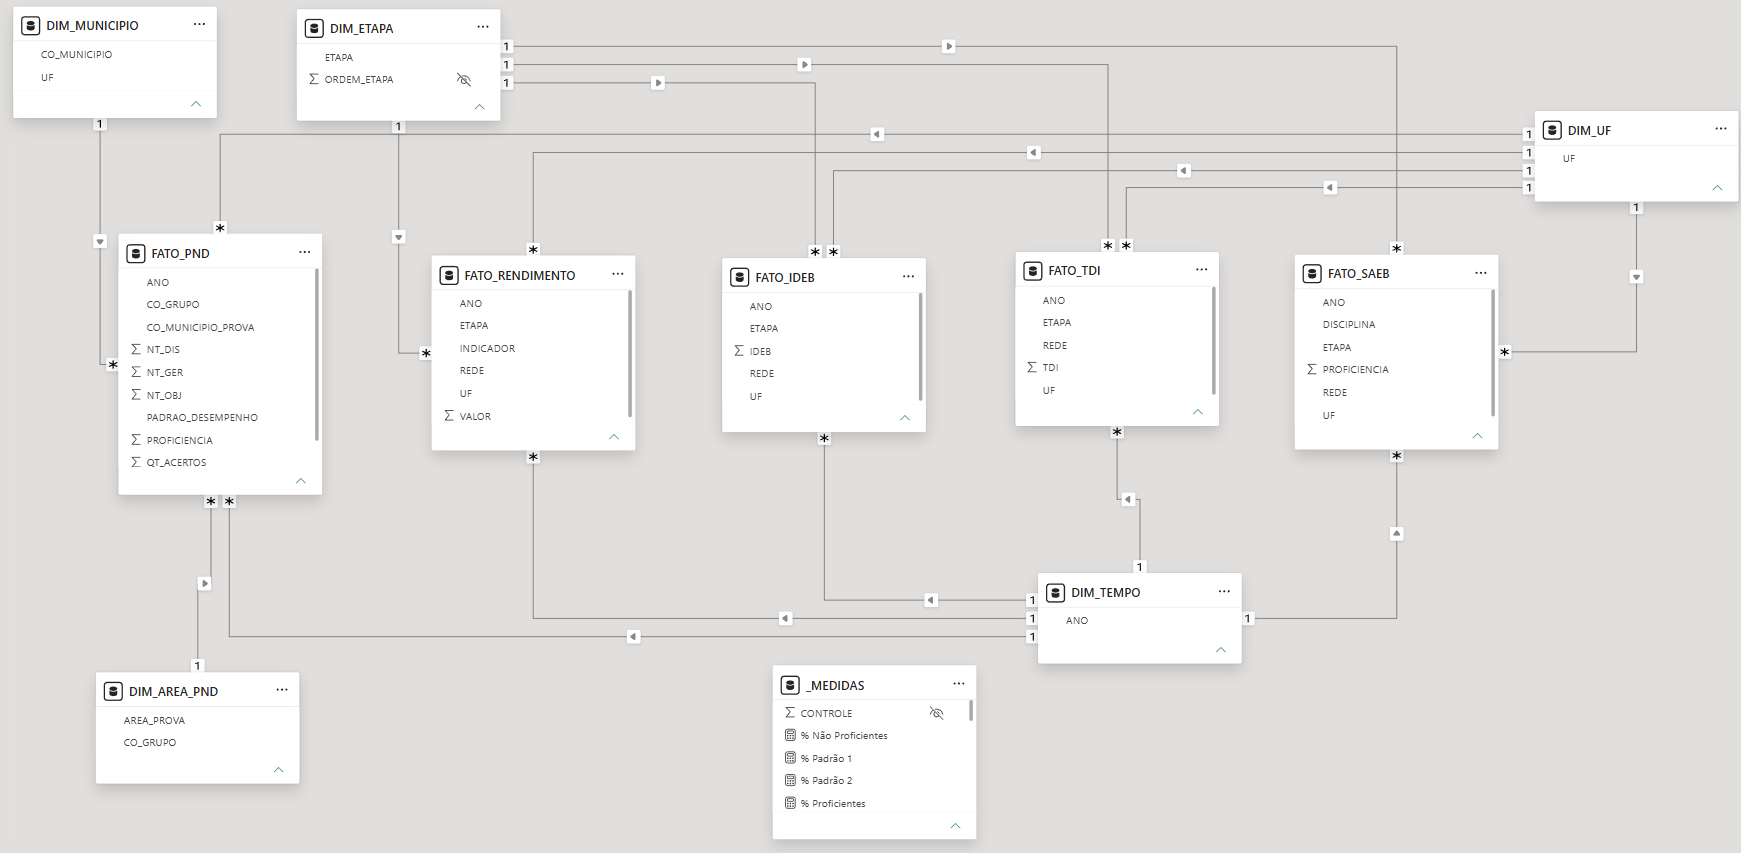
\includegraphics[width=0.95\linewidth]{figs/modelo-dimensional.png}
   \caption{Modelo dimensional atual consumido pelo Power BI.}
   \label{fig:modelo-dimensional}
\end{figure}
\end{landscape}

Na Figura~\ref{fig:modelo-dimensional}, a tabela \texttt{\_MEDIDAS} funciona apenas como contêiner técnico para organizar as medidas DAX no modelo semântico. Ela não constitui uma sexta dimensão nem uma tabela fato analítica.

\section{Desenvolvimento das métricas analíticas}

O modelo semântico possui 27 medidas DAX. As medidas calculam médias, taxas, contagens, proporções, apoio à seleção de anos comparáveis e variações temporais. A Tabela~\ref{tab:medidas-dax} resume os nomes implementados no arquivo \texttt{powerbi/medidas\_power\_bi.dax}.

\begin{table}[H]
\centering
\scriptsize
\caption{Medidas DAX implementadas no modelo semântico.}
\label{tab:medidas-dax}
\renewcommand{\arraystretch}{1.2}
\begin{tabular}{|p{3.0cm}|p{10.0cm}|}
\hline
\textbf{Grupo} & \textbf{Medidas} \\ \hline
Rendimento & \texttt{Taxa de Aprovação}; \texttt{Taxa de Reprovação}; \texttt{Taxa de Abandono} \\ \hline
TDI e IDEB & \texttt{TDI Média}; \texttt{IDEB Médio} \\ \hline
SAEB & \texttt{Proficiência Média SAEB}; \texttt{Proficiência Média LP}; \texttt{Proficiência Média MT} \\ \hline
PND -- médias e contagens & \texttt{Participantes PND}; \texttt{Nota Objetiva Média}; \texttt{Nota Discursiva Média}; \texttt{Nota Geral Média}; \texttt{Média de Acertos}; \texttt{Não Proficientes}; \texttt{Padrão 1}; \texttt{Padrão 2}; \texttt{Proficientes} \\ \hline
PND -- percentuais & \texttt{\% Proficientes}; \texttt{\% Não Proficientes}; \texttt{\% Padrão 1}; \texttt{\% Padrão 2} \\ \hline
Apoio & \texttt{Ano de Avaliação Disponível} \\ \hline
Variações & \texttt{Variação Aprovação}; \texttt{Variação IDEB}; \texttt{Variação SAEB Matemática}; \texttt{Variação SAEB Português}; \texttt{Variação TDI} \\ \hline
\end{tabular}
\legend{Fonte: Elaborado pelo autor a partir do modelo Power BI do projeto (2026).}
\end{table}

As taxas de Rendimento e a TDI já são armazenadas na escala de 0 a 100. Os percentuais da PND são razões calculadas dinamicamente e formatadas como percentuais. As medidas de variação representam diferença absoluta entre o último e o primeiro ano com dado no intervalo selecionado. Suas unidades dependem do indicador: pontos de IDEB, pontos percentuais para Aprovação e TDI e pontos de proficiência para SAEB.

\section{Desenvolvimento dos dashboards}

O Power BI consome exclusivamente os arquivos Parquet da Gold. O Power Query é utilizado como camada de conexão com esses arquivos; relacionamentos, medidas DAX e visualizações compõem o modelo semântico e a apresentação analítica.

A primeira página, \textit{Panorama dos Indicadores da Educação Básica}, reúne cartões de IDEB, proficiência média do SAEB em Matemática e Língua Portuguesa, Aprovação, Reprovação, Abandono e TDI, além das respectivas evoluções históricas.

A segunda página, \textit{Desempenho educacional por Unidade Federativa}, compara as UFs em quatro rankings: IDEB, SAEB Matemática, TDI e SAEB Língua Portuguesa. O ano é selecionado entre avaliações disponíveis para IDEB e SAEB, permitindo comparação territorial dentro de um mesmo recorte temporal.

A terceira página, \textit{Aprendizagem e fluxo escolar por Unidade Federativa}, combina a evolução histórica de Aprovação, Reprovação, Abandono e TDI com dois gráficos de dispersão: Aprovação versus IDEB e Aprovação versus proficiência média do SAEB.

A quarta página, \textit{Variação dos indicadores por Unidade Federativa}, utiliza um intervalo de anos e apresenta as diferenças entre o primeiro e o último ano com dado para IDEB, Aprovação, SAEB Língua Portuguesa e SAEB Matemática, respeitando as unidades próprias de cada indicador.

A quinta página, \textit{Distorção idade-série por Unidade Federativa}, apresenta TDI média e Variação TDI, evolução temporal, comparação por UF, comparação entre Anos Iniciais e Anos Finais e variação territorial.

A sexta página, \textit{Resultados da PND 2025}, apresenta os cartões \texttt{Participantes PND}, \texttt{\% Proficientes}, \texttt{Nota Objetiva Média} e \texttt{Nota Geral Média}. Os gráficos mostram percentual de proficientes por área, percentual de proficientes por UF, nota objetiva média por área e distribuição dos padrões de desempenho por UF. Os filtros visíveis dessa página são UF e área.

A sétima página, \textit{Metodologia e Arquitetura do Projeto}, sintetiza escopo, fontes, arquitetura Raw--Bronze--Silver--Gold--Power BI, modelo dimensional, decisões metodológicas e controles de qualidade. Ela funciona como documentação interna do próprio dashboard.

\begin{landscape}
\begin{figure}[H]
  \centering
  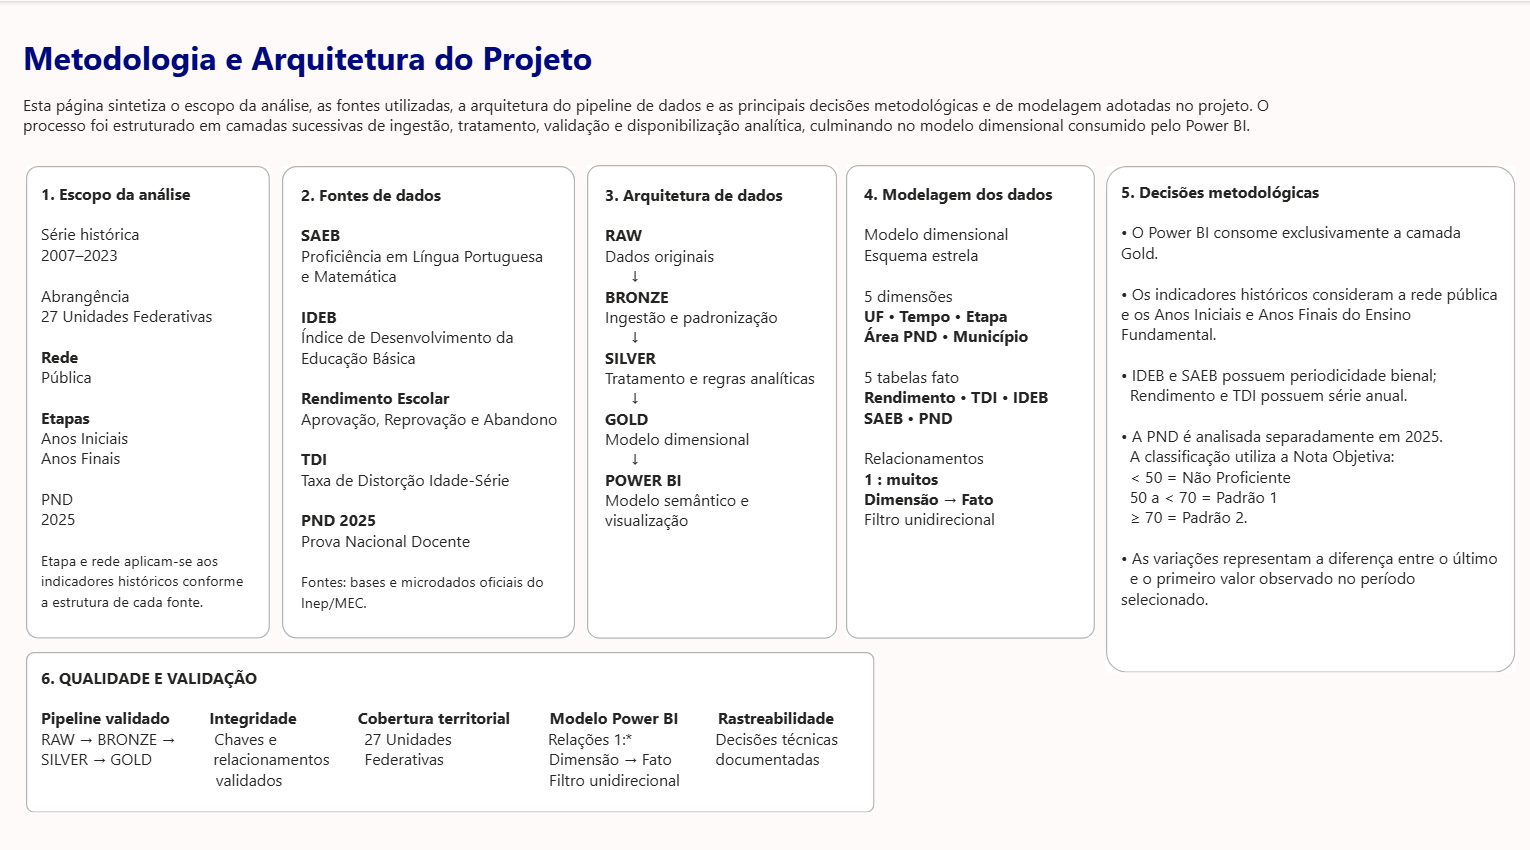
\includegraphics[width=0.95\linewidth]{figs/dashboard-metodologia.png}
  \caption{Página de metodologia e arquitetura do projeto no Power BI.}
  \label{fig:dashboard-metodologia}
\end{figure}
\end{landscape}

\section{Notebooks, testes e automação}

O repositório possui cinco notebooks demonstrativos, um para cada indicador: Rendimento Escolar, TDI, IDEB, SAEB e PND. Eles apresentam o percurso entre a fonte Raw e a tabela fato Gold correspondente e chamam os scripts oficiais do repositório, sem reimplementar as regras de transformação. Assim, os notebooks funcionam como material demonstrativo e executável da metodologia, enquanto a implementação oficial permanece em \texttt{src/}.

Além das validações analíticas, o projeto possui testes automatizados do contrato do repositório e um fluxo de integração contínua para verificações estruturais que não dependem da disponibilidade da Raw. O comando \texttt{python src/pipeline.py full --dry-run} valida a sequência de scripts sem executar as transformações, enquanto o manifesto pode ser verificado independentemente por \texttt{python scripts/gerar\_manifesto\_raw.py --check}.

\section{Ferramentas utilizadas}

Foram utilizadas Python e as bibliotecas registradas no arquivo \texttt{requirements.txt}, incluindo Pandas, NumPy, PyArrow e mecanismos de leitura de planilhas em diferentes formatos. Parquet foi adotado nas camadas derivadas para armazenamento tabular. Também foram utilizados Git para versionamento, notebooks Jupyter como material demonstrativo, Power BI Desktop para o modelo semântico e os dashboards, Power Query para conexão à Gold e DAX para as medidas analíticas.

Essa separação de responsabilidades mantém o processamento reprodutível fora da ferramenta de visualização: Python executa e valida o pipeline; os Parquets constituem a interface analítica; e o Power BI concentra relacionamentos, medidas dependentes do contexto de filtro e visualizações.

\section{Limitações metodológicas}
\label{sec:limitacoes-metodologicas}

As fontes apresentam diferenças históricas de formato, layout, nomenclatura, nível de agregação e semântica das categorias. Essas diferenças exigem regras específicas por indicador e por edição e limitam a interpretação de uma série como se todos os anos fossem metodologicamente idênticos.

A análise histórica é harmonizada principalmente no nível de Unidade Federativa, rede pública e Anos Iniciais/Anos Finais. Portanto, os resultados não devem ser generalizados para escolas ou municípios. No SAEB, as categorias de rede de 2007 e 2009 diferem das edições posteriores. IDEB e SAEB possuem periodicidade bienal, enquanto Rendimento e TDI são anuais.

As médias exibidas no Power BI são médias das linhas existentes no contexto de filtro. Quando diversas UFs são agregadas, esses valores não equivalem automaticamente a uma média nacional ponderada por matrículas ou participantes. Essa distinção é especialmente importante ao interpretar os cartões gerais.

A PND corresponde apenas a 2025 e não constitui série temporal. As variáveis territoriais representam o local de aplicação da prova, não residência. A classificação por padrões utiliza \texttt{NT\_OBJ} e descreve proficiência segundo os pontos de corte adotados; ela não equivale a aprovação ou reprovação.

A reprodução exata depende dos arquivos identificados no manifesto e pelos hashes SHA-256. Novas edições oficiais podem alterar nomes, layouts ou endereços de download, motivo pelo qual a documentação das fontes deve ser considerada em conjunto com o inventário versionado.

Por fim, os dashboards têm finalidade descritiva e exploratória. Associações visuais entre indicadores não permitem estabelecer relações causais nem atribuir mudanças observadas a políticas, condições socioeconômicas ou outros fatores sem desenho de pesquisa específico para inferência causal.


% ----------------------------------------------------------
% Resultados
% ----------------------------------------------------------

\chapter[Resultados e Discussão]{Resultados e Discussão}

Este capítulo apresenta os resultados técnicos e analíticos obtidos com o pipeline e com os dashboards desenvolvidos no Power BI. Os resultados possuem caráter descritivo e exploratório. Assim, as comparações permitem observar padrões, diferenças territoriais e mudanças temporais, mas não sustentam, por si só, inferências causais.

\section{Estrutura final do modelo analítico}

O primeiro resultado é a consolidação das cinco fontes em um modelo dimensional para consumo analítico. A Gold é composta por cinco tabelas fato e cinco dimensões, validadas antes da conexão com o Power BI. As cardinalidades finais são apresentadas na Tabela~\ref{tab:cardinalidades-gold}.

\begin{table}[H]
\centering
\caption{Cardinalidades validadas da camada Gold.}
\label{tab:cardinalidades-gold}
\begin{tabular}{|l|r|}
\hline
\textbf{Tabela} & \textbf{Registros} \\ \hline
\texttt{DIM\_UF} & 27 \\ \hline
\texttt{DIM\_TEMPO} & 18 \\ \hline
\texttt{DIM\_ETAPA} & 2 \\ \hline
\texttt{DIM\_AREA\_PND} & 17 \\ \hline
\texttt{DIM\_MUNICIPIO} & 750 \\ \hline
\texttt{FATO\_RENDIMENTO} & 2.754 \\ \hline
\texttt{FATO\_TDI} & 918 \\ \hline
\texttt{FATO\_IDEB} & 486 \\ \hline
\texttt{FATO\_SAEB} & 972 \\ \hline
\texttt{FATO\_PND} & 759.140 \\ \hline
\end{tabular}
\legend{Fonte: Validação da camada Gold do projeto (2026).}
\end{table}

Foram verificados esquema, domínios, cobertura temporal, unicidade no grão, correspondência entre Silver e Gold, chaves órfãs e coerência entre município e UF. A validação global retornou \texttt{MODELO DIMENSIONAL GOLD: OK}. Esse resultado não atesta a qualidade substantiva das fontes oficiais, mas demonstra que as regras implementadas e os contratos estruturais definidos pelo projeto foram satisfeitos.

\section{Panorama geral dos indicadores educacionais}

A Figura~\ref{fig:dashboard-panorama} apresenta a visão geral dos indicadores históricos. Na captura sem filtros adicionais, os cartões exibem IDEB médio de 4,5, proficiência média de 223,2 em Matemática e 215,4 em Língua Portuguesa, Taxa de Aprovação de 87,5, Taxa de Reprovação de 9,5, Taxa de Abandono de 3,0 e TDI média de 24,9.

Esses valores devem ser interpretados como médias das linhas presentes no contexto do modelo, e não como médias nacionais ponderadas por matrícula. O principal interesse do painel está na leitura conjunta das trajetórias. O IDEB apresenta trajetória visual predominantemente ascendente entre as edições observadas; as proficiências médias de Matemática e Língua Portuguesa também crescem ao longo de grande parte da série, embora com oscilações nas edições mais recentes. A aprovação cresce no período, enquanto a TDI apresenta redução expressiva ao longo dos anos.

A leitura conjunta sugere melhora simultânea em diferentes dimensões do recorte analisado. IDEB e SAEB, porém, são observados em edições bienais, enquanto Rendimento e TDI possuem série anual, o que exige cautela nas comparações temporais.

\begin{figure}[H]
  \centering
  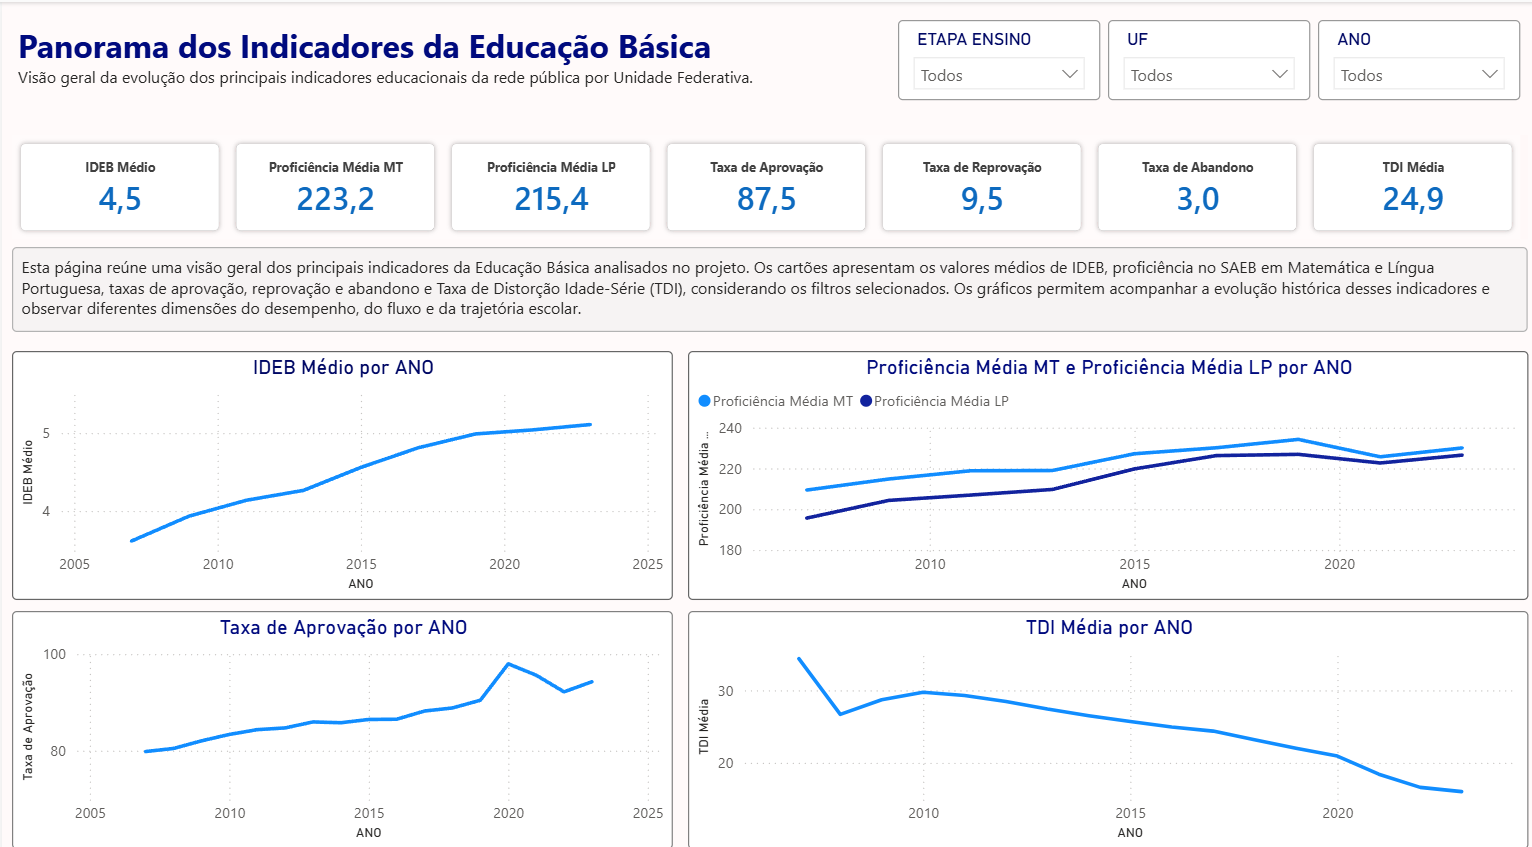
\includegraphics[width=0.98\textwidth]{figs/dashboard-panorama.png}
  \caption{Panorama dos indicadores da Educação Básica.}
  \label{fig:dashboard-panorama}
\end{figure}

\section{Desempenho educacional por Unidade Federativa}

A segunda página compara IDEB, SAEB Matemática, TDI e SAEB Língua Portuguesa entre Unidades Federativas em um ano de avaliação disponível. Na captura da Figura~\ref{fig:dashboard-uf}, o ano selecionado é 2007 e a etapa está em \textit{Todos}.

Nesse recorte, Paraná, Santa Catarina e São Paulo aparecem com IDEB médio de 4,4 entre as barras visíveis. No SAEB, o Distrito Federal aparece no topo visível tanto em Matemática, com 228,4 pontos, quanto em Língua Portuguesa, com 213,0 pontos. Para TDI, Pará e Alagoas aparecem entre os maiores valores visíveis, com 50,1 e 49,9, respectivamente. Esses exemplos evidenciam que a posição de uma UF depende do indicador analisado e que desempenho, fluxo e atraso escolar não formam uma única dimensão.

A página utiliza rankings separados para evitar transformar indicadores de escalas e significados distintos em uma medida única. Diferenças territoriais de desempenho também podem coexistir com condições sociais e educacionais distintas. Em um recorte específico do SAEB 2023 para o 5º ano de escolas públicas do Rio Grande do Norte, \citeonline{de2026desigualdades} identificaram diferenças significativas de proficiência entre escolas urbanas e rurais e ressaltaram sua coexistência com características territoriais e socioeconômicas. Embora se trate de outro recorte analítico, o estudo reforça a necessidade de contextualizar a leitura dos rankings.

\begin{figure}[H]
  \centering
  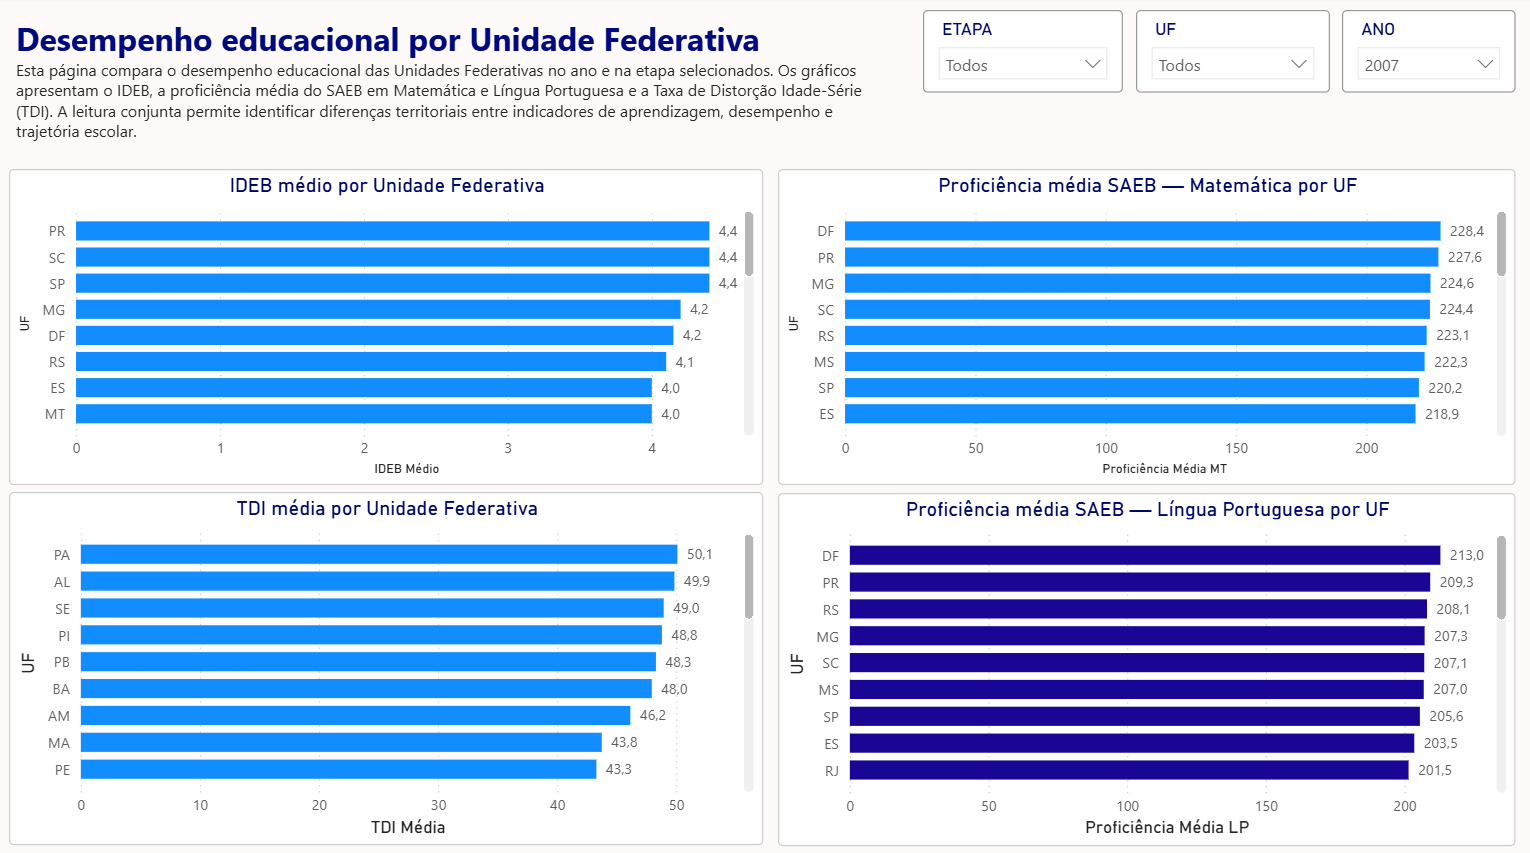
\includegraphics[width=0.98\textwidth]{figs/dashboard-ideb-saeb.png}
  \caption{Desempenho educacional por Unidade Federativa no recorte exibido no dashboard.}
  \label{fig:dashboard-uf}
\end{figure}

\section{Aprendizagem e fluxo escolar}

A página de aprendizagem e fluxo escolar combina duas formas de leitura. Na parte superior, são exibidas séries históricas de Aprovação, Reprovação, Abandono e TDI. Na parte inferior, cada ponto representa uma UF no ano selecionado, relacionando Taxa de Aprovação com IDEB e com proficiência média do SAEB.

Na Figura~\ref{fig:dashboard-aprendizagem-fluxo}, os gráficos históricos mostram aumento da aprovação ao longo do período e redução de TDI, reprovação e abandono em diferentes intensidades. Os gráficos de dispersão, por sua vez, permitem observar associação descritiva entre níveis mais elevados de aprovação e valores mais altos de IDEB ou proficiência em parte das UFs.

O IDEB combina informações de desempenho em avaliações com dados de fluxo escolar em sua composição \cite{inep2024ideb}, o que torna esperada alguma proximidade entre aprovação e IDEB. \citeonline{dias2026avaliaccao} ressaltam que, embora o IDEB seja um instrumento relevante de diagnóstico e planejamento, sua condição de indicador sintético exige interpretação contextualizada, evitando reduzir a complexidade educacional a uma única medida. A dispersão entre aprovação e proficiência do SAEB, por sua vez, deve ser lida apenas como associação descritiva.

\begin{figure}[H]
  \centering
  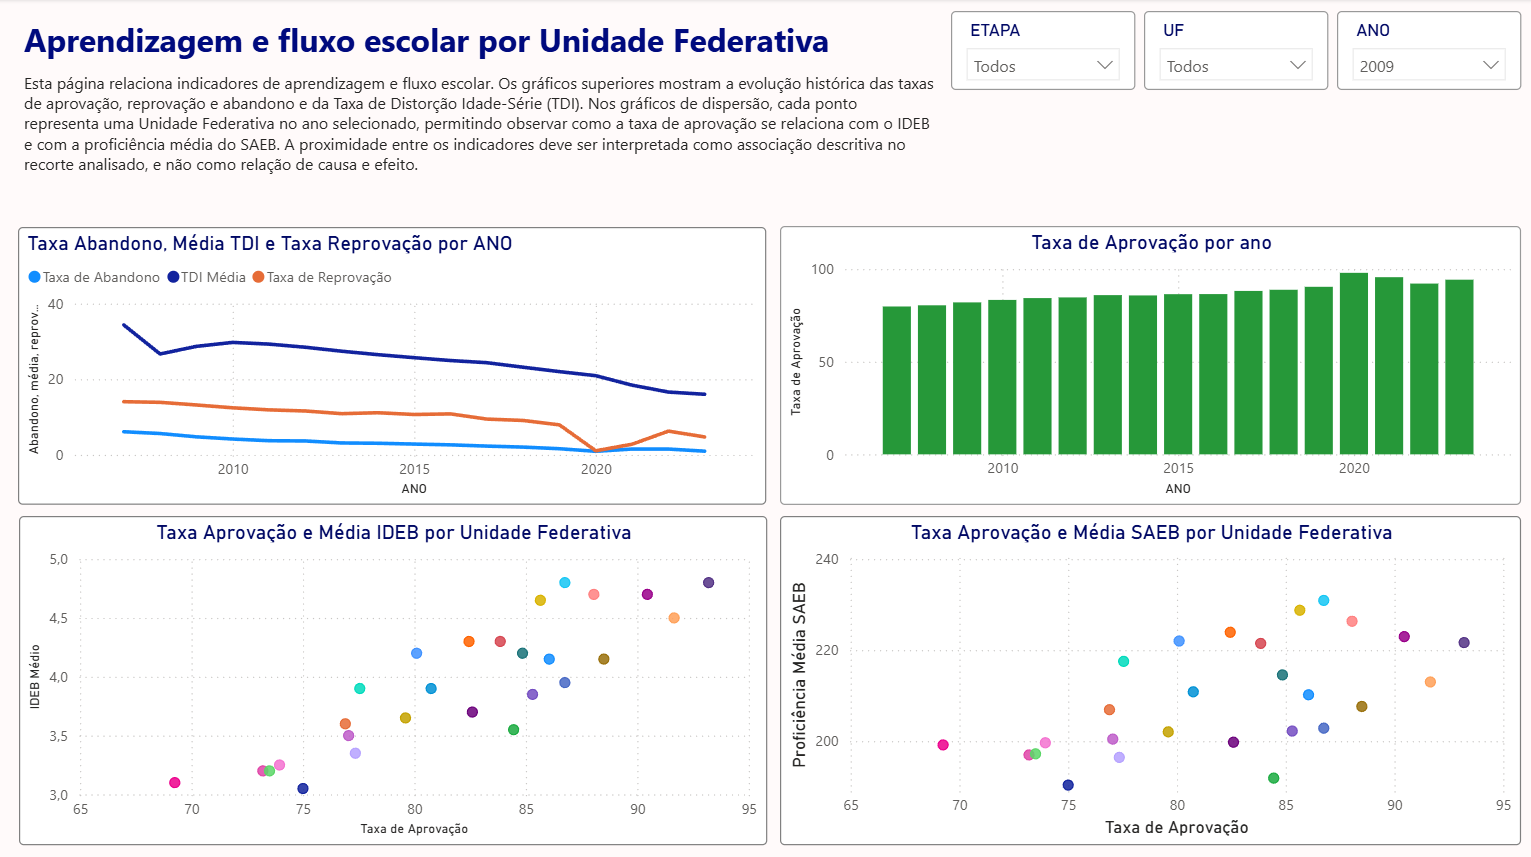
\includegraphics[width=0.98\textwidth]{figs/dashboard-aprendizagem-fluxo.png}
  \caption{Aprendizagem e fluxo escolar por Unidade Federativa.}
  \label{fig:dashboard-aprendizagem-fluxo}
\end{figure}

\section{Variação dos indicadores por Unidade Federativa}

As medidas de variação comparam o último e o primeiro ano com dado disponível dentro do intervalo selecionado para cada indicador. Isso evita supor observações anuais onde a fonte é bienal. As unidades também diferem: IDEB é expresso em pontos do índice; Aprovação, em pontos percentuais; e SAEB, em pontos de proficiência.

Na Figura~\ref{fig:dashboard-variacao}, o intervalo selecionado é 2007--2023. Entre as barras visíveis, Ceará apresenta a maior variação de IDEB, com 2,6 pontos, e também a maior variação de proficiência em Língua Portuguesa, com 60 pontos, além de 51 pontos em Matemática. Na Taxa de Aprovação, Alagoas aparece com aumento de 27 pontos percentuais. Esses valores descrevem diferença entre extremos observados no período e não uma taxa de crescimento relativa.

As diferenças territoriais reforçam que a evolução não ocorre de forma uniforme entre as UFs.

\begin{figure}[H]
  \centering
  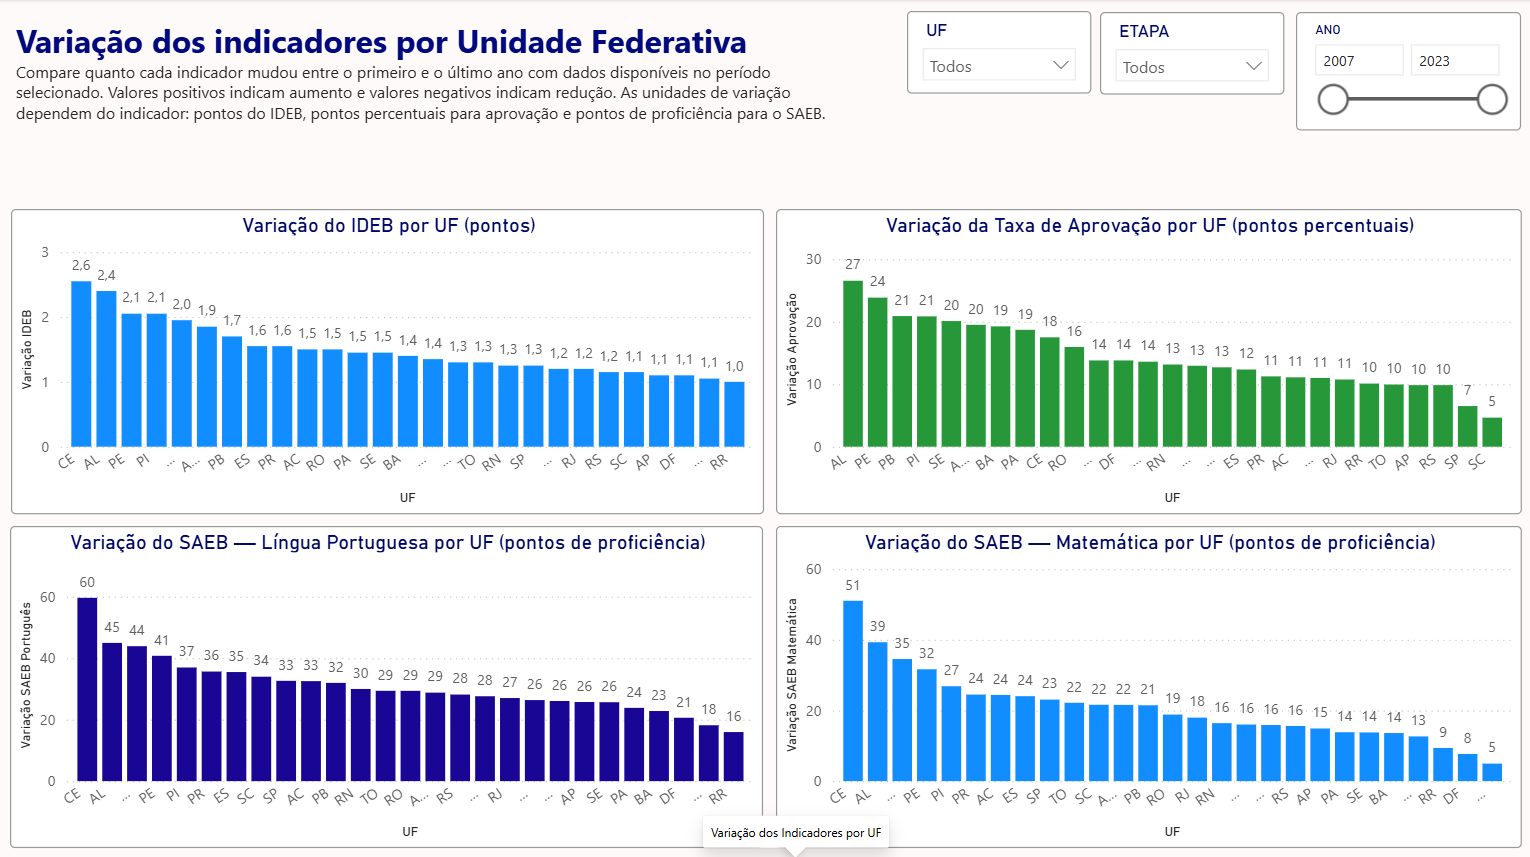
\includegraphics[width=0.98\textwidth]{figs/dashboard-variacao.png}
  \caption{Variação dos indicadores por Unidade Federativa no intervalo 2007--2023.}
  \label{fig:dashboard-variacao}
\end{figure}

\section{Análise da Taxa de Distorção Idade-Série}

A Figura~\ref{fig:dashboard-tdi} apresenta a TDI em quatro perspectivas: evolução anual, média por UF, média por etapa de ensino e variação por UF. No intervalo 2007--2023 mostrado no painel, a TDI média é 24,9 e a Variação TDI é -18,3 pontos percentuais.

A evolução temporal passa de 34,4 no início da série exibida para 16,0 em 2023. Por etapa, os Anos Finais apresentam TDI média de 32,3, enquanto os Anos Iniciais apresentam 17,5. No ranking de médias por UF, Sergipe aparece com 37,2 e São Paulo com 8,6 nos extremos visíveis do painel. A variação territorial é negativa para todas as barras exibidas, indicando redução da distorção no intervalo considerado, embora em magnitudes diferentes entre as UFs.

A redução é um resultado favorável sob a interpretação do indicador, pois a TDI expressa a proporção de estudantes em situação de distorção entre idade e série \cite{inep2026tdi}; portanto, valores menores indicam menor incidência dessa condição no recorte analisado. Contudo, a permanência de médias elevadas em determinadas UFs e a diferença entre etapas mostram que o problema não desaparece de forma homogênea. \citeonline{leal2025distorccao} discute a distorção idade-série como um fenômeno associado a fatores pedagógicos, sociais e estruturais, entre eles repetência e vulnerabilidade socioeconômica, aspectos que não são modelados pelo dashboard.

\begin{figure}[H]
  \centering
  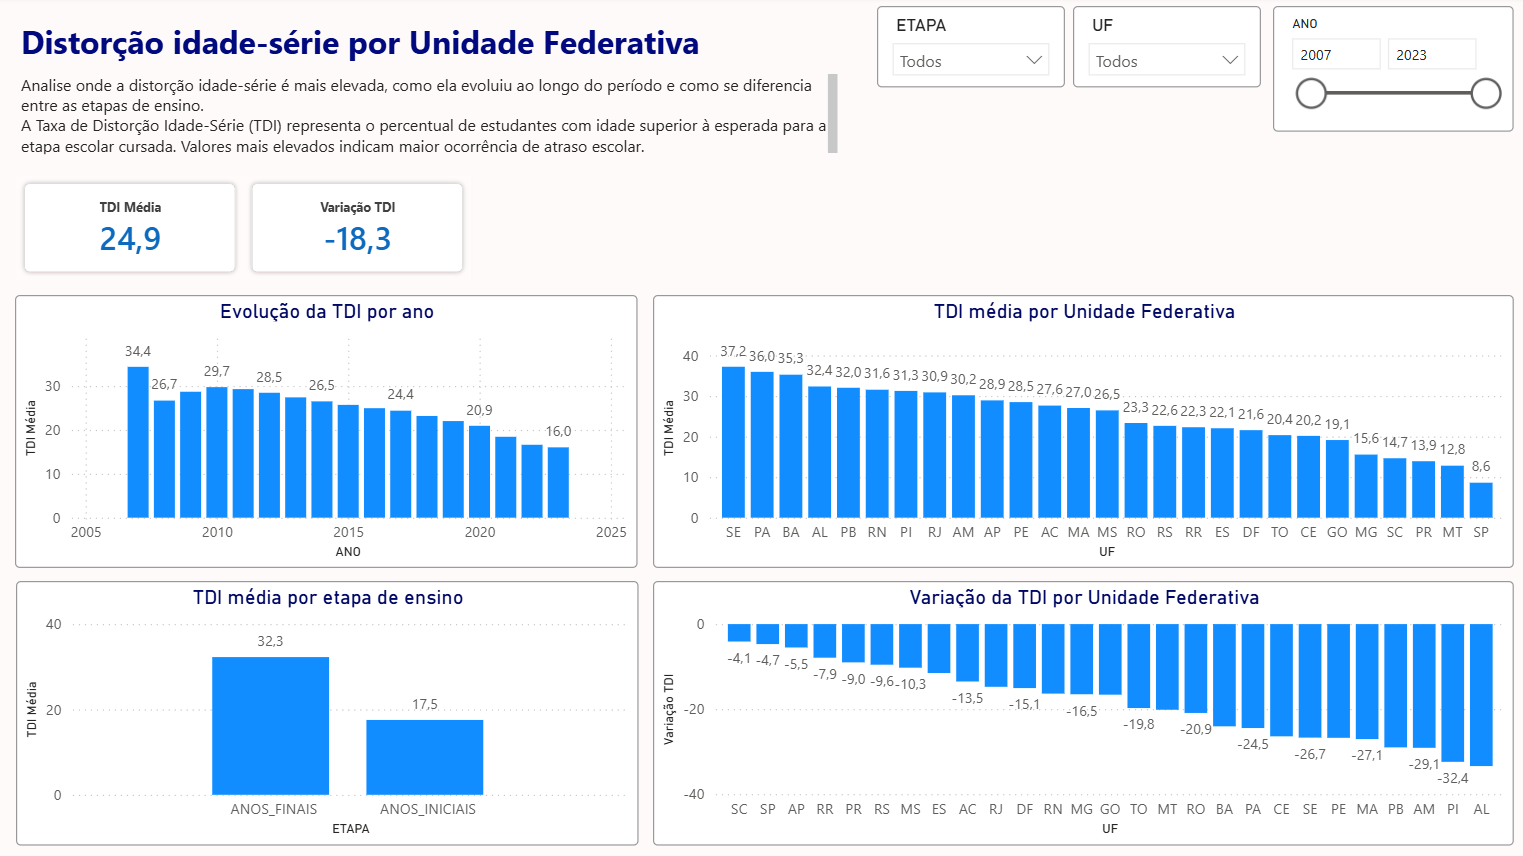
\includegraphics[width=0.98\textwidth]{figs/dashboard-tdi.png}
  \caption{Distorção idade-série por Unidade Federativa e etapa de ensino.}
  \label{fig:dashboard-tdi}
\end{figure}

\section{Resultados da PND 2025}

A PND é analisada separadamente das séries históricas. A população analítica contém 759.140 registros. A classificação utilizada no projeto é baseada em \texttt{NT\_OBJ} e nos pontos de corte documentados para a PND \cite{inep2025notatecnica44,inep2026notatecnica1}. Aplicando essa regra à população analítica, obtiveram-se 265.932 não proficientes, 304.638 participantes no Padrão 1 e 188.570 no Padrão 2. A soma dos padrões 1 e 2 corresponde a 493.208 proficientes, equivalentes a 64,97\% da população analítica.

Na Figura~\ref{fig:dashboard-pnd}, os cartões arredondam esse resultado para 759 mil participantes e 65,0\% de proficientes. A Nota Objetiva Média exibida é 57,5 e a Nota Geral Média é 57,3. Os gráficos complementam a leitura com percentual de proficientes por área, percentual de proficientes por UF, nota objetiva média por área e distribuição dos três padrões por UF.

A classificação deve ser interpretada nos termos dos pontos de corte aplicados à nota objetiva \cite{inep2025notatecnica44,inep2026notatecnica1}. Não se trata de aprovação ou reprovação e o limite de 50 pontos não representa simplesmente 50\% de acertos. A distribuição por UF e área também é descritiva da população analítica da prova. Como \texttt{UF\_PROVA} representa a Unidade Federativa de aplicação, diferenças territoriais não devem ser interpretadas automaticamente como características de residência dos participantes.

\begin{figure}[H]
  \centering
  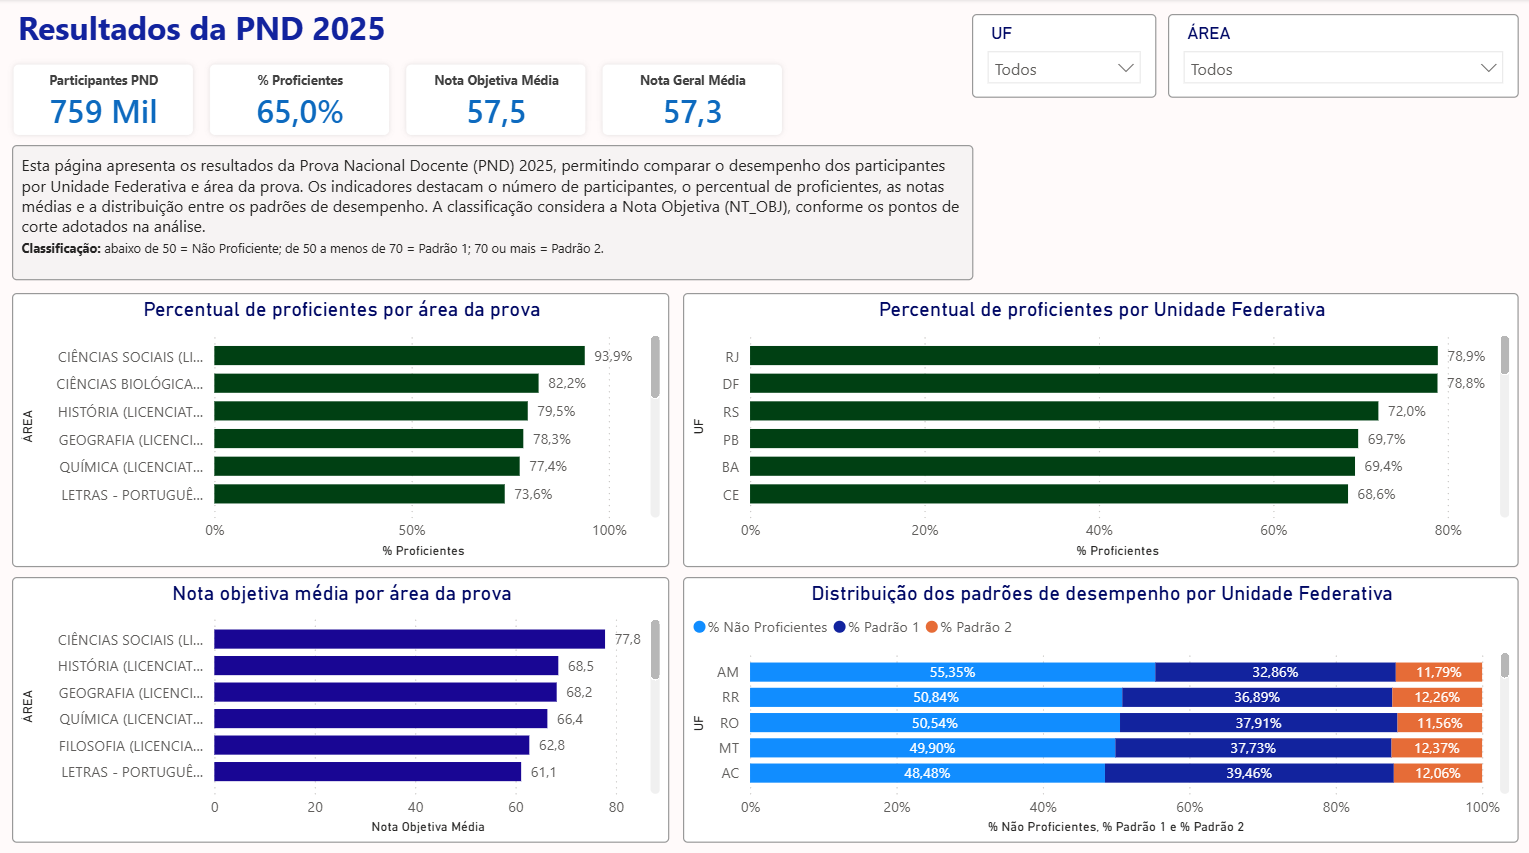
\includegraphics[width=0.98\textwidth]{figs/dashboard-pnd-medias.png}
  \caption{Resultados da Prova Nacional Docente de 2025.}
  \label{fig:dashboard-pnd}
\end{figure}

\section{Limitações observadas nos resultados}

Os resultados devem ser lidos em conjunto com as limitações metodológicas apresentadas na Seção~\ref{sec:limitacoes-metodologicas}. Em particular, as fontes diferem em periodicidade, nível de agregação e categorias históricas, enquanto a análise foi harmonizada principalmente por UF, rede pública e etapa de ensino.

Os cartões de média no Power BI calculam a média das linhas presentes no contexto de filtro. Quando todas as UFs estão selecionadas, esse valor não equivale automaticamente a um indicador nacional ponderado por matrícula ou por quantidade de participantes. Assim, os números gerais do dashboard devem ser interpretados como sínteses do modelo analítico construído, e não como substitutos de estatísticas nacionais oficiais produzidas com outros ponderadores.

Por fim, nenhuma associação visual apresentada neste capítulo deve ser interpretada como relação de causa e efeito. O projeto foi desenhado para integração, rastreabilidade e exploração descritiva dos dados; investigações causais exigiriam desenho metodológico, variáveis de controle e técnicas estatísticas específicas.


% ---
% Finaliza a parte no bookmark do PDF, para que se inicie o bookmark na raiz
% ---
\bookmarksetup{startatroot}%
% ---

% ---
% Conclusão
% ---
\chapter[Conclusão]{Conclusão}

Este trabalho investigou como uma arquitetura reprodutível de Engenharia de Dados pode integrar bases educacionais heterogêneas do INEP e disponibilizá-las de forma consistente para análise no Power BI. A questão de pesquisa foi respondida por meio da construção de um pipeline em Python organizado nas camadas Raw, Bronze, Silver e Gold, acompanhado de manifesto das fontes, hashes SHA-256, metadados de linhagem, validadores independentes e uma camada analítica consumida exclusivamente pelo Power BI.

O pipeline integrou IDEB, SAEB, Rendimento Escolar e TDI no recorte histórico de 2007 a 2023 e incorporou a PND 2025 como análise complementar. A solução final materializou cinco tabelas fato e cinco dimensões. A validação global confirmou a integridade estrutural do modelo e as correspondências definidas entre as camadas, retornando \texttt{MODELO DIMENSIONAL GOLD: OK}.

A construção mostrou que a integração de fontes oficiais exige mais do que reunir arquivos em uma ferramenta de visualização. Foi necessário tratar diferenças de formato, layout, periodicidade, granularidade e semântica de rede, além de documentar decisões específicas por indicador. No SAEB, por exemplo, a preservação dos agregados oficiais de UF evitou substituir o valor publicado por uma recomposição escolar que não reproduzia o resultado oficial. Na PND, a auditoria da população e o uso dos pontos de corte aplicados à \texttt{NT\_OBJ} substituíram critérios analíticos anteriores e produziram uma classificação coerente com a documentação adotada no projeto.

O Power BI atuou como camada de consumo e análise. As 27 medidas DAX e as páginas do dashboard permitiram observar panorama histórico, desempenho por Unidade Federativa, associação descritiva entre aprendizagem e fluxo, variações territoriais, distorção idade-série e resultados da PND 2025. As medidas temporais foram implementadas de forma a usar o primeiro e o último ano com dado dentro do intervalo selecionado, respeitando a periodicidade anual de Rendimento e TDI e a periodicidade bienal de IDEB e SAEB.

Os resultados descritivos evidenciam trajetórias distintas entre indicadores e UFs. No panorama geral do modelo, observam-se aumento do IDEB, das proficiências e da aprovação ao longo de grande parte da série, acompanhado de redução da TDI. Na página específica de TDI, o intervalo 2007--2023 apresenta variação média de -18,3 pontos percentuais no contexto exibido, enquanto a PND reúne 759.140 participantes e 493.208 classificados como proficientes, correspondentes a 64,97\% da população analítica. Esses resultados são descritivos e não demonstram relações causais.

A principal contribuição técnica do trabalho está na reprodutibilidade do percurso entre fonte e consumo analítico. O inventário de 54 arquivos Raw, a identificação por hashes, a documentação da origem, os validadores de cada camada, o orquestrador e os testes do repositório tornam explícitas decisões que, em um fluxo restrito à ferramenta de BI, poderiam permanecer ocultas. Os notebooks demonstrativos complementam essa documentação, sem substituir os scripts oficiais do pipeline.

As limitações permanecem relevantes. A série histórica é harmonizada principalmente em nível de UF, rede pública e etapas agregadas, o que impede inferências sobre escolas ou municípios. As fontes possuem metodologias e layouts que mudam ao longo do tempo; SAEB apresenta particularidade de rede em 2007 e 2009; IDEB e SAEB são bienais; a PND possui apenas 2025; e as médias do dashboard não equivalem automaticamente a médias nacionais ponderadas. Além disso, as visualizações não permitem inferência causal.

Dessa forma, conclui-se que a arquitetura desenvolvida atingiu o objetivo proposto: bases públicas heterogêneas foram integradas em um pipeline documentado, validado e rastreável, chegando a um modelo dimensional consistente para exploração no Power BI. A contribuição do trabalho está tanto no produto analítico final quanto na explicitação do processo de Engenharia de Dados necessário para produzi-lo.

\section{Principais Contribuições}

As principais contribuições podem ser sintetizadas em cinco eixos. Primeiro, a integração de fontes educacionais heterogêneas do INEP em um fluxo único. Segundo, a arquitetura em camadas, que separa preservação, ingestão, harmonização e consumo analítico. Terceiro, a rastreabilidade e a reprodutibilidade, apoiadas por manifesto, hashes, linhagem, validadores, testes e orquestração. Quarto, a modelagem dimensional com cinco fatos e cinco dimensões. Quinto, a disponibilização dos dados em um modelo semântico com 27 medidas DAX e dashboards temáticos.

No componente territorial, a padronização histórica por Unidade Federativa viabilizou a integração entre fontes com diferentes estruturas. Para a PND, o modelo preservou também o código do município de aplicação e a relação ativa com \texttt{DIM\_MUNICIPIO}, sem criar uma relação direta entre essa dimensão e \texttt{DIM\_UF}, evitando ambiguidade de filtro.

A incorporação da PND 2025 demonstrou a possibilidade de integrar uma fonte de granularidade individual ao mesmo ambiente analítico sem tratá-la como continuação artificial da série histórica da Educação Básica. A separação entre a análise histórica e a PND preservou a interpretação de cada fonte.

\section{Trabalhos Futuros}

Como trabalhos futuros, sugere-se ampliar o modelo com outras bases do INEP, como Censo Escolar, infraestrutura, matrículas, turmas e formação docente. A inclusão dessas fontes pode permitir análises adicionais, desde que cada nova base passe pelo mesmo processo de auditoria, documentação de fonte, harmonização e validação.

Outra possibilidade é aprofundar a granularidade territorial ou institucional. O presente trabalho prioriza UFs na análise histórica; pesquisas futuras podem desenvolver recortes municipais ou escolares quando houver compatibilidade de fonte, grão e metodologia.

Também podem ser incorporados indicadores socioeconômicos de instituições como IBGE ou IPEA. Essa expansão permitiria explorar associações mais amplas entre contexto social e indicadores educacionais, sem confundir análise descritiva com inferência causal.

Em estudos futuros, técnicas estatísticas ou de ciência de dados podem ser utilizadas para correlação, regressão, agrupamento ou séries temporais. Caso o objetivo seja investigar causalidade, será necessário um desenho específico de pesquisa, com hipóteses, controles e métodos adequados.

No caso da PND, novas edições poderão permitir a construção de uma série própria, separada dos indicadores históricos deste trabalho. Também é possível evoluir a publicação do dashboard para ambiente institucional ou público, com atenção a usabilidade, atualização automatizada e governança dos dados.

\section{Contribuições em Produção Bibliográfica}

Até o momento da finalização deste trabalho, não houve publicação de artigo científico resultante diretamente da pesquisa. O projeto, entretanto, oferece material para futuras produções sobre pipelines reprodutíveis de dados educacionais, qualidade e linhagem de dados públicos, modelagem dimensional aplicada ao INEP, integração de indicadores da Educação Básica e visualização analítica em Power BI.

Possíveis trabalhos derivados incluem estudos sobre reprodutibilidade de pipelines educacionais, comparação de metodologias de publicação entre edições do SAEB, integração de indicadores históricos com novas fontes e uso de visualizações para comunicação de resultados educacionais.





% ----------------------------------------------------------
% ELEMENTOS PÓS-TEXTUAIS
% ----------------------------------------------------------
\postextual

% ----------------------------------------------------------
% Referências bibliográficas
% ----------------------------------------------------------
\bibliography{bib/abntex2-modelo-references}

% ----------------------------------------------------------
% Glossário
% ----------------------------------------------------------
%
%\glossary

% ----------------------------------------------------------
% Apêndices
% ----------------------------------------------------------
% ---
% Inicia os apêndices
% ---
%\begin{apendicesenv}
% Imprime uma página indicando o início dos apêndices
%\partapendices
% ----------------------------------------------------------
% Incluir Apêndice
% ----------------------------------------------------------
%\end{apendicesenv}
% ---

% ----------------------------------------------------------
% Anexos
% ----------------------------------------------------------
% ---
% Inicia os anexos
% ---
%\begin{anexosenv}
% Imprime uma página indicando o início dos anexos
%\partanexos
% ---
% Incluir Anexo
% ---
%\chapter{Morbi ultrices rutrum lorem.}

%o comando lipsum[] comando serve apenas para incluir texto no documento para efeito de visualização do formato.
%\lipsum[1-25]
%\section{Test}
%\lipsum[1-20]


%\end{anexosenv}


\end{document}
